\chapter{Subcellular Localisation of IFIT2 in the Context of RSV Inclusion Bodies} \label{ch:Subcellular Localisation of IFIT2 in the Context of RSV Inclusion Bodies}
\section{Introduction and Aims} \label{sec:Introduction and Aims-Chapter5}
Talk about the two antibodies

\section{Results} \label{sec:Results-Chapter5}
\subsection{IFIT2 Subcellular Localisation During Interferon Induction and RSV
Infection} \label{subsec:IFIT2 Subcellular Localisation During Interferon Induction and RSV
Infection}
antibody validation plots

\lipsum[1-5]


\subsection{IFIT2(A) Localisation in the Context of RSV pIBs and IBs} \label{subsec:IFIT2(A) Localisation in the Context of RSV pIBs and IBs}
\subsubsection{IFIT2(A) in a Simplified System of pseudo-IBs} \label{IFIT2(A) in a Simplified System of pseudo-IBs}
%Nascent Human and Monkey IFIT2 in pIBs
%i2a 293t hnhp
Cell Line: 293T \newline
Treatment: hNhP \newline
Detecting magenta: endogenous human IFIT2 \newline
Detecting cyan: human pIB \newline

Nascent human IFIT2 strongly concentrates within the human RSV pseudo inclusion bodies.

\begin{figure}
    \centering
    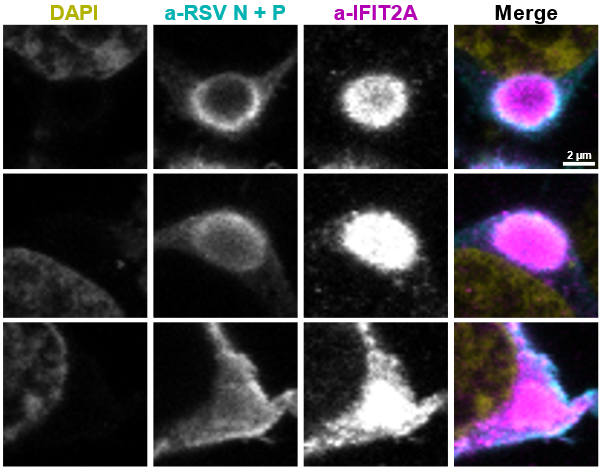
\includegraphics[width=1\linewidth]{10. Chapter 5//Figs//01. I2A/01. i2a 293t hnhp.png}
    \caption[i2a 293t hnhp]{i2a 293t hnhp}
    \label{fig:i2a 293t hnhp}
\end{figure}

%i2a vero hnhp
Cell Line: VERO \newline
Treatment: hNhP \newline
Detecting magenta: endogenous monkey IFIT2 \newline
Detecting cyan: human pIB \newline

Endogenous monkey IFIT2 colocalises with the pIB structure (probably like an inclusion), as well as with the pIB filamentous network.

\begin{figure}
    \centering
    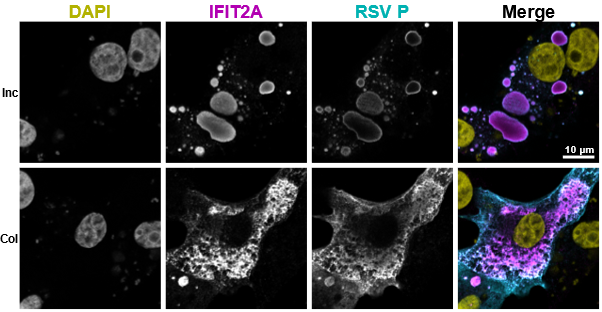
\includegraphics[width=1\linewidth]{10. Chapter 5//Figs//01. I2A/02. i2a vero hnhp.png}
    \caption[i2a vero hnhp]{i2a vero hnhp}
    \label{fig:i2a vero hnhp}
\end{figure}

%Exogenous Human and Bovine IFIT2 in pBs
%i2a vero hi2 + hnhp
Cell Line: VERO \newline
Treatment: hNhP + hIFIT2-FLAG \newline
Detecting magenta: endogenous monkey IFIT2 + exogenous human IFIT2 \newline
Detecting cyan: human pIB \newline

Monkey cells transfected with human RSV N and P, along with human IFIT2-FLAG show concentration within the pIB structures as well as the pIB filamentous network. In this experiment we are detecting both human and monkey IFIT2, however we can see a huge difference in IFIT2 expression between some cells (bottom panel; cells in the periphery of the picture), suggesting that what we are mainly detecting is the overexpressed human IFIT2-FLAG.

\begin{figure}
    \centering
    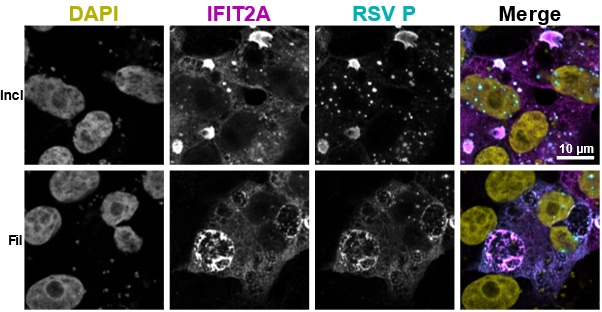
\includegraphics[width=1\linewidth]{10. Chapter 5//Figs//01. I2A/03. i2a vero hi2 hnhp.png}
    \caption[i2a vero hi2 + hnhp]{i2a vero hi2 + hnhp}
    \label{fig:i2a vero hi2 + hnhp}
\end{figure}

\subsubsection{Nascent IFIT2(A) Localisation in the Context of IBs} \label{Nascent IFIT2(A) Localisation in the Context of IBs}
%hIFIT2A localisation during hRSV Infection
%i2a a549 hrsv
Cell Line: A549 \newline
Treatment: hRSV \newline
Detecting magenta: endogenous human IFIT2  \newline
Detecting cyan: human IB \newline

Nascent human IFIT2 shows 3 phenotypes with regards to colocalization with human RSV N. It seems to colocalise to the edge of the IB structure, with a partial signal also being detected in the inner edge of the structure (top panel); it completely colocalises to the N staining (middle panel; could be because the section is going through the top of the IB sphere); or forms inclusion inside the IB structure (bottom panel. 

\begin{figure}
    \centering
    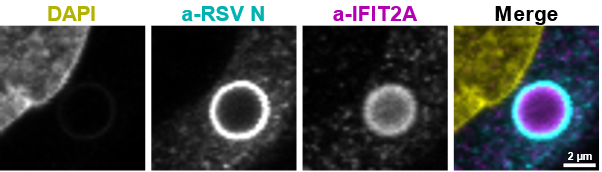
\includegraphics[width=1\linewidth]{10. Chapter 5//Figs//01. I2A/04. i2a a549 hrsv n.png}
    \caption[i2a a549 hrsv n]{i2a a549 hrsv n}
    \label{fig:i2a a549 hrsv n}
\end{figure}

Cell Line: A549 \newline
Treatment: hRSV \newline
Detecting magenta: endogenous human IFIT2  \newline
Detecting cyan: human IB \newline

Nascent human IFIT2 colocalises with the ring structure (outlined by RSV P staining) and to the inner edge of the IB.

\begin{figure}
    \centering
    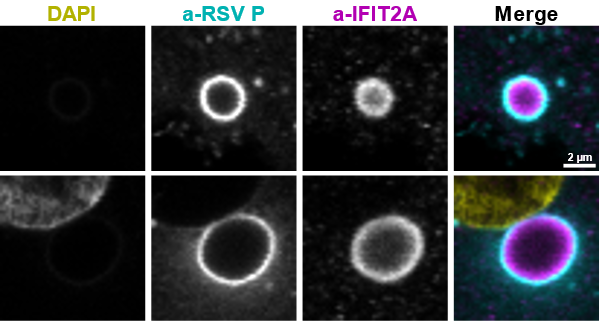
\includegraphics[width=1\linewidth]{10. Chapter 5//Figs//01. I2A/05. i2a a549 hrsv p.png}
    \caption[i2a a549 hrsv p]{i2a a549 hrsv p}
    \label{fig:i2a a549 hrsv p}
\end{figure}

Cell Line: A549 \newline
Treatment: hRSV \newline
Detecting magenta: endogenous human IFIT2  \newline
Detecting cyan: human IB \newline

With regards of colocalization with human RSV M2/1 protein, human IFIT2 seems to either form inclusion, which has a signal decrease towards the middle of the IB structure (top panel), or seems to strongly colocalise with the ring structure highlighted by M2/1 staining (bottom 2 panels; there also seems to be IFIT2 signal concentration on the inner edge of the IB structure).

\begin{figure}
    \centering
    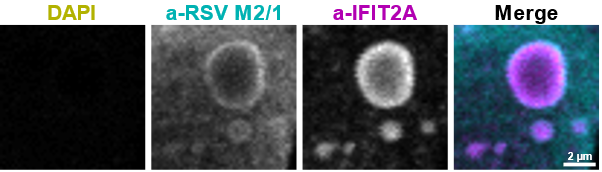
\includegraphics[width=1\linewidth]{10. Chapter 5//Figs//01. I2A/06. i2a a549 hrsv m21.png}
    \caption[i2a a549 hrsv m21]{i2a a549 hrsv m21}
    \label{fig:i2a a549 hrsv m21}
\end{figure}

%i2a beas2b hrsv
Cell Line: BEAS2B \newline
Treatment: hRSV \newline
Detecting magenta: endogenous human IFIT2  \newline
Detecting cyan: human IB \newline

\begin{figure}
    \centering
    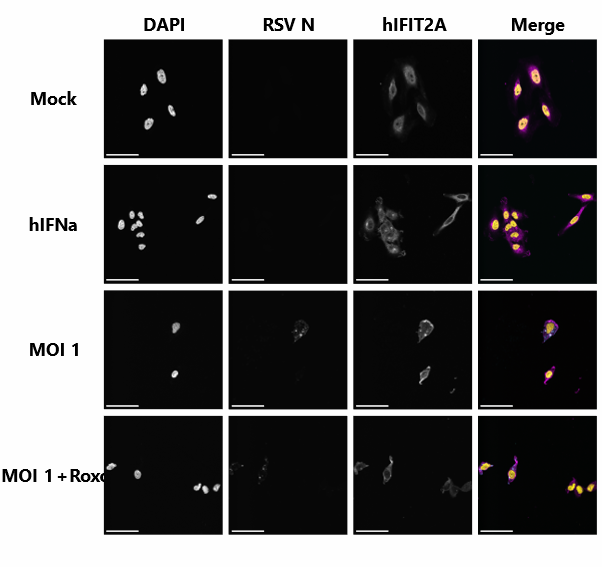
\includegraphics[width=1\linewidth]{10. Chapter 5//Figs//01. I2A/07. i2a beas2b hrsv.png}
    \caption[i2a beas2b hrsv]{i2a beas2b hrsv}
    \label{fig:i2a beas2b hrsv}
\end{figure}

%hIFIT2A localisation during bRSV Infection
%i2a mdbk brsv
Cell Line: MDBK \newline
Treatment: bRSV + bIFNa \newline
Detecting magenta: endogenous bovine IFIT2  \newline
Detecting cyan: bovine IB \newline

Nascent bovine IFIT2 colocalization with regards of N stained bRSV IBs seems to strongly associate with the ring of the structure.

\begin{figure}
    \centering
    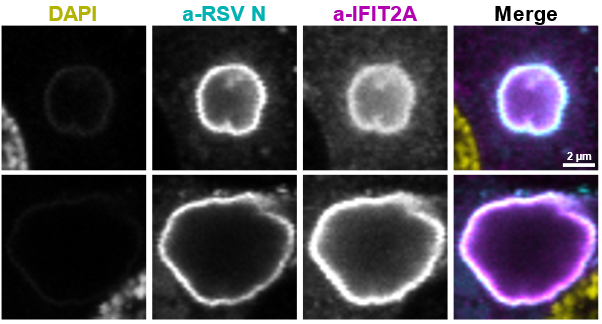
\includegraphics[width=1\linewidth]{10. Chapter 5//Figs//01. I2A/08. i2a mdbk brsv.png}
    \caption[i2a mdbk brsv]{i2a mdbk brsv}
    \label{fig:i2a mdbk brsv}
\end{figure}

\subsubsection{Summary} \label{Summary-i2a}
Both endogenous human and monkey IFIT2 forms inclusions inside human RSV pseudo-IBs. Monkey IFIT2 also colocalises to the pIB filamentous network (this structure was not observed in the human experiment). The identical staining can be observed in monkey cells with overexpressed human IFIT2-FLAG. Nascent human IFIT2 during hRSV infection consistently localises to the IB structure. It seems to have preference for the ring and the inner edge of the structure; however, we have seen it as homogenous inclusion as well. Endogenous bovine IFIT2 colocalises to the ring of the IB during bRSV infection.
\subsection{IFIT2B} \label{subsec:IFIT2B}
IFIT2B -> stuff detected by anti-IFIT2 antibody B

Everything stated in this subchapter is only attributable to the staining seen with IFIT2 antibody B
\subsubsection{Nascent Human and Monkey IFIT2 in a Simplified System of pseudo-IBs} \label{Nascent Human and Monkey IFIT2 in a Simplified System of pseudo-IBs}
\myparagraph{Nascent Human and Monkey IFIT2 in pIBs}
\mysubparagraph{i2b vero hnhp}
Cell Line: VERO \newline
Treatment: hNhP \newline
Detecting magenta: endogenous monkey IFIT2 \newline
Detecting cyan: human pIB \newline

Nascent monkey IFIT2 is completely excluded from the human RSV pseudo-IBs and the pIB filamentous network.

\begin{figure}
    \centering
    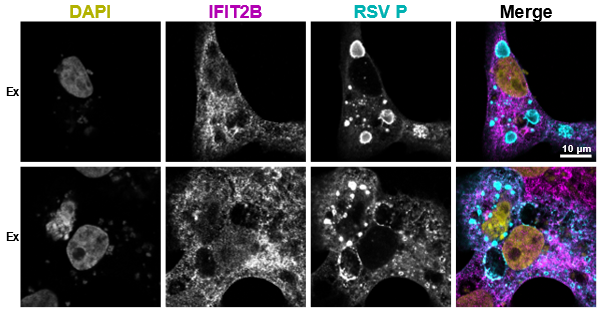
\includegraphics[width=1\linewidth]{10. Chapter 5//Figs//02. I2B/01. i2b vero hnhp.png}
    \caption[i2b vero hnhp]{i2b vero hnhp}
    \label{fig:i2b vero hnhp}
\end{figure}

\myparagraph{Exogenous Human and Bovine IFIT2 in pBs}
\mysubparagraph{i2b vero hi2 + hnhp}
Cell Line: VERO \newline
Treatment: hNhP + hIFIT2-FLAG \newline
Detecting magenta: endogenous monkey IFIT2 + exogenous human IFIT2 \newline
Detecting cyan: human pIB \newline

Monkey cells transfected with human RSV N and P, along with human IFIT2-FLAG show concentration within the pIB structures but show exclusion from the pIB filamentous network (or partial colocalsiation?). This suggest that the IFIT2B antibody can indeed detect IFIT2 but the overexpressed IFIT2 observed between the inclusion and the one interacting with the filamentous network is somehow different (epitope masking?).

\begin{figure}
    \centering
    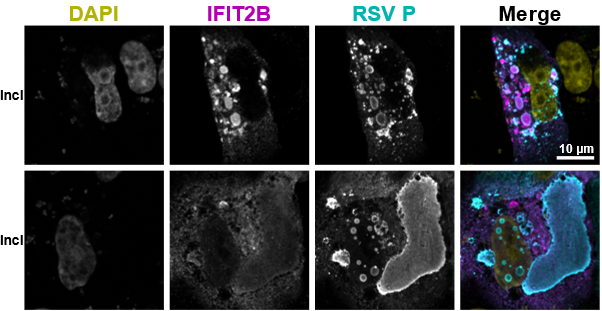
\includegraphics[width=1\linewidth]{10. Chapter 5//Figs//02. I2B/02. i2b vero i2 hnhp.png}
    \caption[i2b vero hi2 + hnhp]{i2b vero hi2 + hnhp}
    \label{fig:i2b vero hi2 + hnhp}
\end{figure}

\subsubsection{Nascent Human and Bovine IFIT2B Localisation During h/bRSV Infection} \label{Nascent Human and Bovine IFIT2B Localisation During h/bRSV Infection}
\myparagraph{hIFIT2B localisation during hRSV Infection}
\mysubparagraph{i2b a549 hrsv}
Cell Line: A549 \newline
Treatment: hRSV \newline
Detecting magenta: endogenous human IFIT2  \newline
Detecting cyan: human IB \newline

Endogenous human IFIT2 is either partially excluded (top panel; decrease of intra IB signal compared to cytoplasmic signal) or completely excluded (bottom panel) from the human IB structure.

\begin{figure}
    \centering
    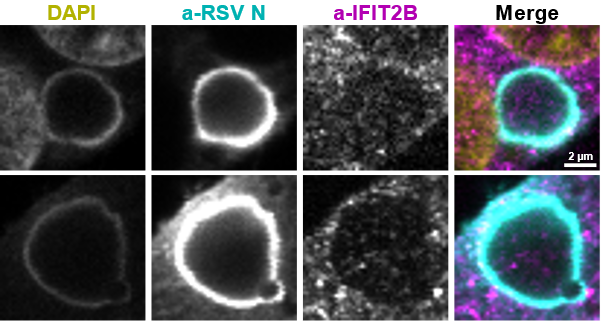
\includegraphics[width=1\linewidth]{10. Chapter 5//Figs//02. I2B/03. i2b a549 hrsv n.png}
    \caption[i2b a549 hrsv n]{i2b a549 hrsv n}
    \label{fig:i2b a549 hrsv n}
\end{figure}

Cell Line: A549 \newline
Treatment: hRSV \newline
Detecting magenta: endogenous human IFIT2  \newline
Detecting cyan: human IB  \newline

We observe similar pattern of staining to what was observed with N stained human IBs. IFIT2 signal is either partially or totally excluded from the IB structure.

\begin{figure}
    \centering
    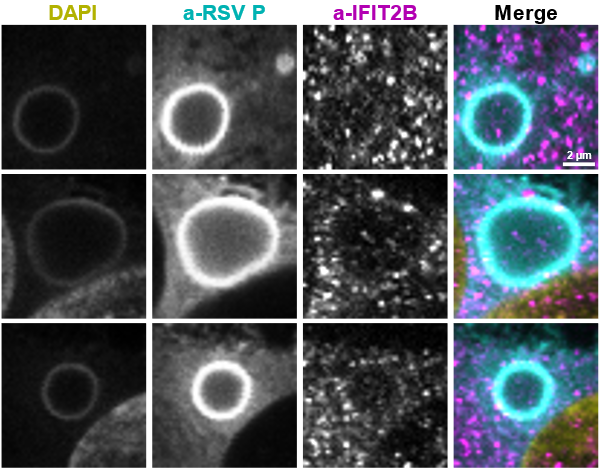
\includegraphics[width=1\linewidth]{10. Chapter 5//Figs//02. I2B/04. i2b a549 hrsv p.png}
    \caption[i2b a549 hrsv p]{i2b a549 hrsv p}
    \label{fig:i2b a549 hrsv p}
\end{figure}

Cell Line: A549 \newline
Treatment: hRSV \newline
Detecting magenta: endogenous human IFIT2  \newline
Detecting cyan: human IB \newline

Endogenous human IFIT2 seems to be excluded from hRSV IBs.

\begin{figure}
    \centering
    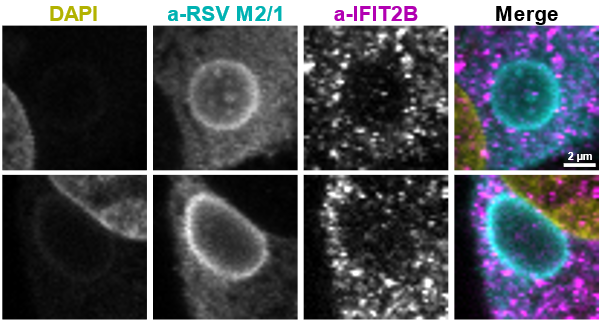
\includegraphics[width=1\linewidth]{10. Chapter 5//Figs//02. I2B/05. i2b a549 hrsv m21.png}
    \caption[i2b a549 hrsv m21]{i2b a549 hrsv m21}
    \label{fig:i2b a549 hrsv m21}
\end{figure}

\mysubparagraph{i2b beas2b hrsv}
some text

\begin{figure}
    \centering
    
\includegraphics[width=0.5\linewidth]{10. Chapter 5//Figs//02. I2B/00. placeholder.png}
    \caption[i2b beas2b hrsv]{i2b beas2b hrsv}
    \label{fig:i2b beas2b hrsv}
\end{figure}

\myparagraph{hIFIT2B localisation during bRSV Infection}
\mysubparagraph{i2b mdbk brsv}
Cell Line: MDBK \newline
Treatment: bRSV + bIFNa \newline
Detecting magenta: endogenous bovine IFIT2  \newline
Detecting cyan: bovine IB \newline

Endogenous bovine IFIT2 localisation with respect to the bovine inclusion bodies shows a few different phenotypes. We see partial exclusion (to panel; signal still present in the middle of the IB structure), exclusion from IB ring and the inner IB edge (middle panel; highlighted with arrow) with IBAG-like concentrations inside the structure; and diffusion through the IB structure (bottom panel). These phenotypes are similar to what is observed during RSV infection of human but especially bovine IFIT3 and IFIT5.

\begin{figure}
    \centering
    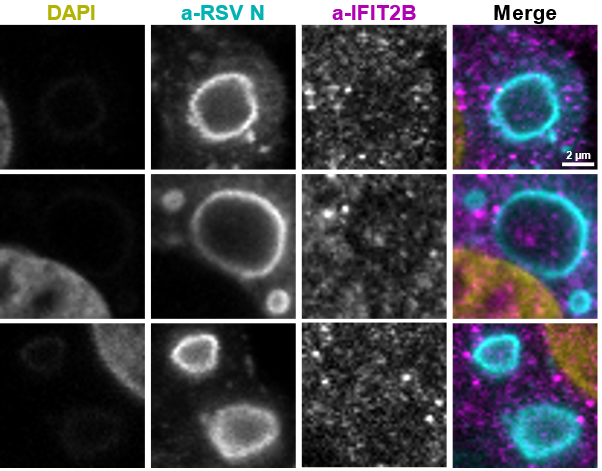
\includegraphics[width=1\linewidth]{10. Chapter 5//Figs//02. I2B/06. i2b mdbk brsv.png}
    \caption[i2b mdbk brsv]{i2b mdbk brsv}
    \label{fig:i2b mdbk brsv}
\end{figure}

\subsection{Summary} \label{subsec:Summary-i2b}
Endogenous monkey IFIT2 is excluded from human pIB and the pIB associated filamentous network. Overexpressed human IFIT2-FLAG is detected by the antibody and shows inclusions inside the human pIB structures, which is consistent to data from IFIT2A staining and FLAG staining of IFIT2-FLAG overexpressed samples. Interestingly, IFIT2B antibody shows exclusion from the pIB filamentous network, which was colocalised by IFIT2A and FLAG antibodies. Nascent human IFIT2 shows full or partial exclusion from human IBs during human RSV infection. Nascent bovine IFIT2 during bRSV infections shows 3 different phenotypes. We observed partial exclusion; exclusion from the IB ring and inner edge with IBAG-like inclusions; and diffusion through the IB structure. This staining is similar to what is observed with bovine IFIT3 and IFIT5 during bRSV infection.
\subsection{Exogenous IFIT2-FLAG Localisation in the Context of RSV pIBs and IBs} \label{subsec:Exogenous IFIT2-FLAG Localisation in the Context of RSV pIBs and IBs}
\subsubsection{IFIT2-FLAG in a Simplified System of pseudo-IBs} \label{IFIT2-FLAG in a Simplified System of pseudo-IBs}
Monkey cells transfected with human RSV N and P, along with human IFIT2-FLAG show concentration within the pIB structures as well as the pIB filamentous network. In this experiment we are detecting both human and monkey IFIT2, however we can see a huge difference in IFIT2 expression between some cells (bottom panel; cells in the periphery of the picture), suggesting that what we are mainly detecting is the overexpressed human IFIT2-FLAG.

\begin{figure}
    \begin{subfigure}{0.495\textwidth}
        \caption{}
        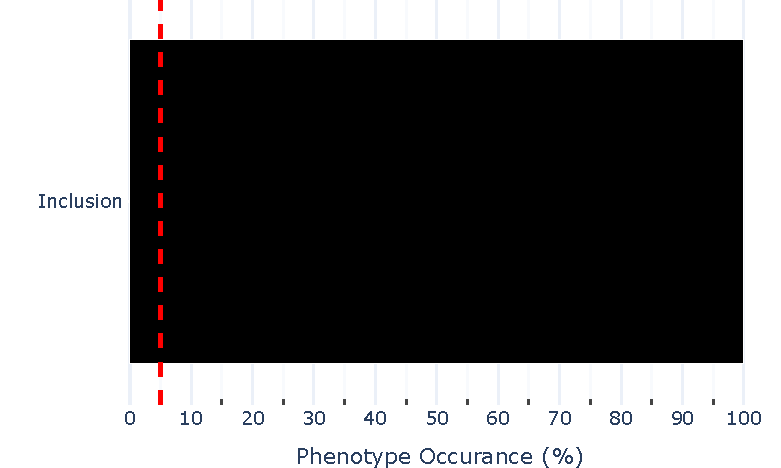
\includegraphics[width=1\linewidth]{10. Chapter 5/Figs/03. IFIT2-FLAG/01. IFIT2A/01. bar_i2a_hnhp.pdf} 
    \end{subfigure}
    \begin{subfigure}{0.495\textwidth}
        \caption{}
        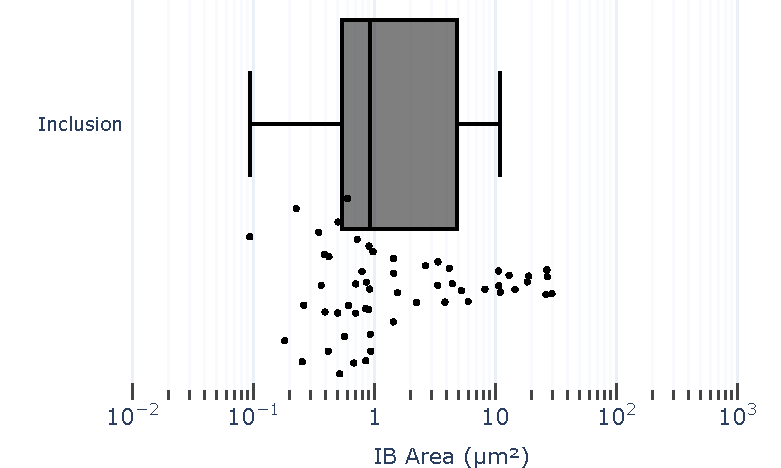
\includegraphics[width=1\linewidth]{10. Chapter 5/Figs/03. IFIT2-FLAG/01. IFIT2A/02. box_i2a_hnhp.pdf}
    \end{subfigure}
    \caption[Observed Phenotypes of Exogenous Human IFIT2 in the Context of hRSV Pseudo Inclusion Bodies in VERO Cell Line, as Detected by IFIT2A Antibody.]{\textbf{Observed Phenotypes of Exogenous Human IFIT2 in the Context of hRSV Pseudo Inclusion Bodies in VERO Cell Line, as Detected by IFIT2A Antibody.} Vero cells were transfected with hRSV N and P, along with human IFIT2-FLAG containing plasmids using TransIT-X2 and were fixed after 24 hours. Cells were labeled with anti-RSV N and anti-IFIT2A antibodies and imaged on confocal microscope. Panel (a) shows percentual proportions of observed phenotypes between hRSV pseudo inclusion bodies and exogenous human IFIT2 (56 observations), with the red dotted line denoting the 5\% threshold, marking phenotypes considered relevant above this limit. Panel (b) shows the IB area in \(\mu m^2\) per observed relevant phenotype.}
    \label{fig:Observed Phenotypes of Exogenous Human IFIT2 in the Context of hRSV Pseudo Inclusion Bodies in VERO Cell Line, as Detected by IFIT2A Antibody}
\end{figure}

\begin{figure}
    \centering
    \includegraphics[width=1\linewidth]{10. Chapter 5/Figs/03. IFIT2-FLAG/01. IFIT2A/03. i2a-hi2f-hnhp.pdf}
    \caption[Representative Images of Observed Phenotypes of Exogenous Human IFIT2 in the Context of hRSV Pseudo Inclusion Bodies in VERO Cell Line, as Detected by IFIT2A Antibody.]{\textbf{Representative Images of Observed Phenotypes of Exogenous Human IFIT2 in the Context of hRSV Pseudo Inclusion Bodies in VERO Cell Line, as Detected by IFIT2A Antibody.} Vero cells were transfected with hRSV N and P, along with human IFIT2-FLAG containing plasmids using TransIT-X2 and were fixed after 24 hours. Cellular nuclei were stained with DAPI (yellow), and cells were double-labeled with anti-RSV N (cyan) and anti-IFIT2A (magenta) antibodies. This figure showcases representative examples of relevant phenotypes in the interaction between exogenous human IFIT2 and hRSV pseudo inclusion bodies. These phenotypes are presented in descending order based on their percentage proportions. The scale bar indicates 2 \(\mu m\).}
    \label{fig:Representative Images of Observed Phenotypes of Exogenous Human IFIT2 in the Context of hRSV Pseudo Inclusion Bodies in VERO Cell Line, as Detected by IFIT2A Antibody}
\end{figure}

Monkey cells transfected with human RSV N and P, along with human IFIT2-FLAG show concentration within the pIB structures but show exclusion from the pIB filamentous network (or partial colocalsiation?). This suggest that the IFIT2B antibody can indeed detect IFIT2 but the overexpressed IFIT2 observed between the inclusion and the one interacting with the filamentous network is somehow different (epitope masking?).

\begin{figure}
    \begin{subfigure}{0.495\textwidth}
        \caption{}
        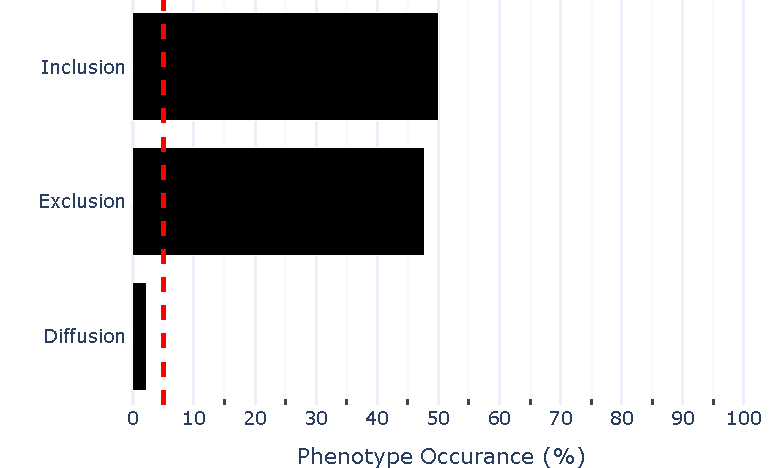
\includegraphics[width=1\linewidth]{10. Chapter 5/Figs/03. IFIT2-FLAG/02. IFIT2B/01. bar_i2b_hnhp.pdf}
    \end{subfigure}
    \begin{subfigure}{0.495\textwidth}
        \caption{}
        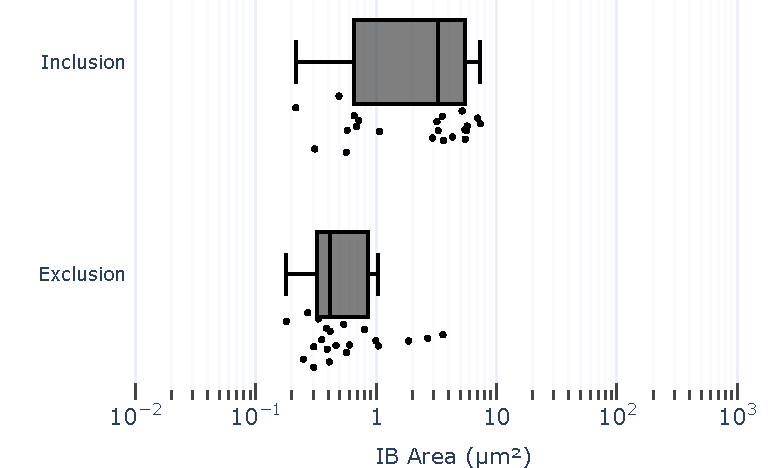
\includegraphics[width=1\linewidth]{10. Chapter 5/Figs/03. IFIT2-FLAG/02. IFIT2B/02. box_i2a_hnhp.pdf}
    \end{subfigure}
    \caption[Observed Phenotypes of Exogenous Human IFIT2 in the Context of hRSV Pseudo Inclusion Bodies in VERO Cell Line, as Detected by IFIT2B Antibody.]{\textbf{Observed Phenotypes of Exogenous Human IFIT2 in the Context of hRSV Pseudo Inclusion Bodies in VERO Cell Line, as Detected by IFIT2B Antibody.} Vero cells were transfected with hRSV N and P, along with human IFIT2-FLAG containing plasmids using TransIT-X2 and were fixed after 24 hours. Cells were labeled with anti-RSV N and anti-IFIT2B antibodies and imaged on confocal microscope. Panel (a) shows percentual proportions of observed phenotypes between hRSV pseudo inclusion bodies and exogenous human IFIT2 (44 observations), with the red dotted line denoting the 5\% threshold, marking phenotypes considered relevant above this limit. Panel (b) shows the IB area in \(\mu m^2\) per observed relevant phenotype.}
    \label{fig:Observed Phenotypes of Exogenous Human IFIT2 in the Context of hRSV Pseudo Inclusion Bodies in VERO Cell Line, as Detected by IFIT2B Antibody}
\end{figure}

\begin{figure}
    \centering
    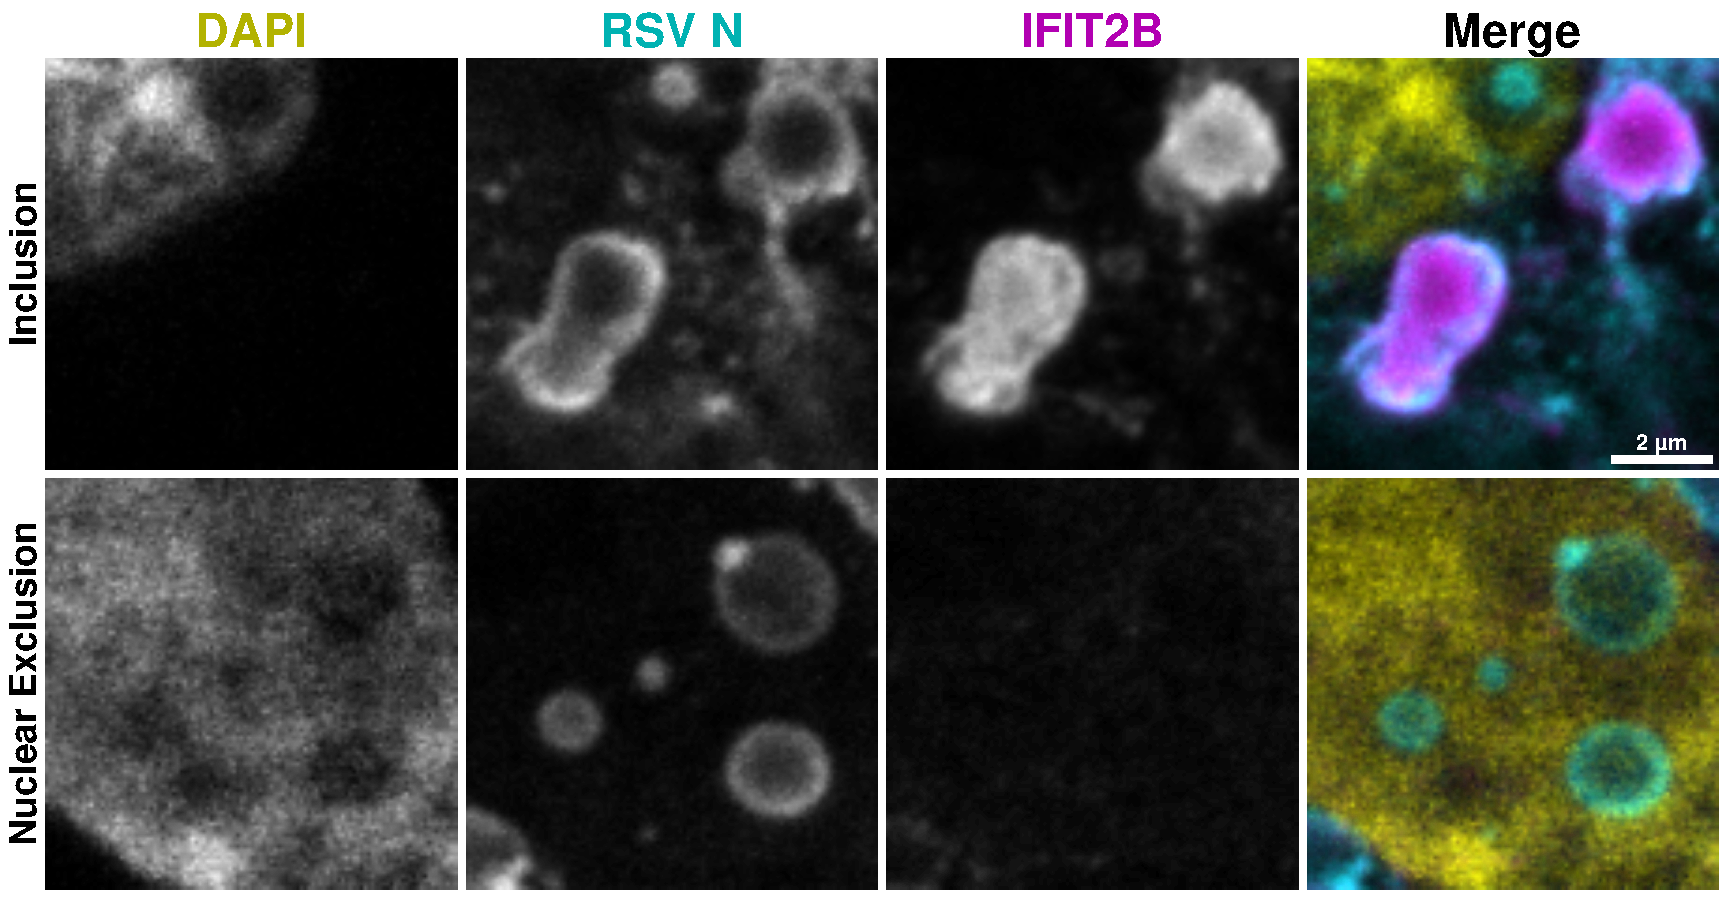
\includegraphics[width=1\linewidth]{10. Chapter 5/Figs/03. IFIT2-FLAG/02. IFIT2B/03. i2b-hi2f-hnhp.pdf}
    \caption[Representative Images of Observed Phenotypes of Exogenous Human IFIT2 in the Context of hRSV Pseudo Inclusion Bodies in VERO Cell Line, as Detected by IFIT2B Antibody.]{\textbf{Representative Images of Observed Phenotypes of Exogenous Human IFIT2 in the Context of hRSV Pseudo Inclusion Bodies in VERO Cell Line, as Detected by IFIT2B Antibody.} Vero cells were transfected with hRSV N and P, along with human IFIT2-FLAG containing plasmids using TransIT-X2 and were fixed after 24 hours. Cellular nuclei were stained with DAPI (yellow), and cells were double-labeled with anti-RSV N (cyan) and anti-IFIT2B (magenta) antibodies. This figure showcases representative examples of relevant phenotypes in the interaction between exogenous human IFIT2 and hRSV pseudo inclusion bodies. These phenotypes are presented in descending order based on their percentage proportions. The scale bar indicates 2 \(\mu m\).}
    \label{fig:Representative Images of Observed Phenotypes of Exogenous Human IFIT2 in the Context of hRSV Pseudo Inclusion Bodies in VERO Cell Line, as Detected by IFIT2B Antibody}
\end{figure}

Exogenously expressed human IFIT2 colocalises with the pIB associated filamentous net (top panel). It also forms inclusion inside the human pIB structures. This data is consistent with what we observed with IFIT2A antibody. IFIT2 also seems to occasionally form aggregates/spots (highlighted by arrows). These could be functional or just aggregates caused by overexpression, we do not know.

\begin{figure}
    \begin{subfigure}{0.495\textwidth}
        \caption{}
        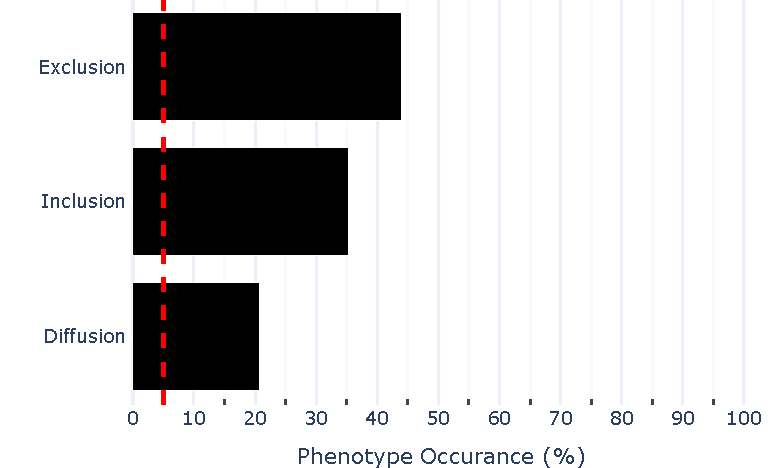
\includegraphics[width=1\linewidth]{10. Chapter 5/Figs/03. IFIT2-FLAG/03. IFIT2F/01. pIB/01. bar_hi2f_hnhp.pdf}
    \end{subfigure}
    \begin{subfigure}{0.495\textwidth}
        \caption{}
        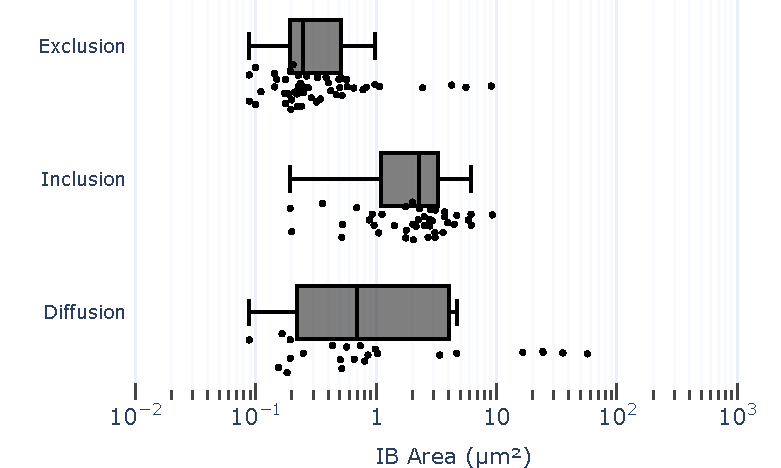
\includegraphics[width=1\linewidth]{10. Chapter 5/Figs/03. IFIT2-FLAG/03. IFIT2F/01. pIB/02. box_hi2f_hnhp.pdf}
    \end{subfigure}
    \caption[Observed Phenotypes of Exogenous Human IFIT2 in the Context of hRSV Pseudo Inclusion Bodies in VERO Cell Line, as Detected by FLAG Antibody.]{\textbf{Observed Phenotypes of Exogenous Human IFIT2 in the Context of hRSV Pseudo Inclusion Bodies in VERO Cell Line, as Detected by FLAG Antibody.} Vero cells were transfected with hRSV N and P, along with human IFIT2-FLAG containing plasmids using TransIT-X2 and were fixed after 24 hours. Cells were labeled with anti-RSV N and anti-FLAG antibodies and imaged on confocal microscope. Panel (a) shows percentual proportions of observed phenotypes between hRSV pseudo inclusion bodies and exogenous human IFIT2 (116 observations), with the red dotted line denoting the 5\% threshold, marking phenotypes considered relevant above this limit. Panel (b) shows the IB area in \(\mu m^2\) per observed relevant phenotype.}
    \label{fig:Observed Phenotypes of Exogenous Human IFIT2 in the Context of hRSV Pseudo Inclusion Bodies in VERO Cell Line, as Detected by FLAG Antibody}
\end{figure}

\begin{figure}
    \centering
    \includegraphics[width=1\linewidth]{10. Chapter 5/Figs/03. IFIT2-FLAG/03. IFIT2F/01. pIB/03. hi2f-hnhp.pdf}
    \caption[Representative Images of Observed Phenotypes of Exogenous Human IFIT2 in the Context of hRSV Pseudo Inclusion Bodies in VERO Cell Line, as Detected by FLAG Antibody.]{\textbf{Representative Images of Observed Phenotypes of Exogenous Human IFIT2 in the Context of hRSV Pseudo Inclusion Bodies in VERO Cell Line, as Detected by FLAG Antibody.} Vero cells were transfected with hRSV N and P, along with human IFIT2-FLAG containing plasmids using TransIT-X2 and were fixed after 24 hours. Cellular nuclei were stained with DAPI (yellow), and cells were double-labeled with anti-RSV N (cyan) and anti-FLAG (magenta) antibodies. This figure showcases representative examples of relevant phenotypes in the interaction between exogenous human IFIT2 and hRSV pseudo inclusion bodies. These phenotypes are presented in descending order based on their percentage proportions. The scale bar indicates 2 \(\mu m\).}
    \label{fig:Representative Images of Observed Phenotypes of Exogenous Human IFIT2 in the Context of hRSV Pseudo Inclusion Bodies in VERO Cell Line, as Detected by FLAG Antibody}
\end{figure}

Exogenous bovine IFIT2 colocalises with the edge of human pIB structures. This is unusual as human IFIT2 data suggest inclusions with regards to pIBs.

\begin{figure}
    \begin{subfigure}{0.495\textwidth}
        \caption{}
        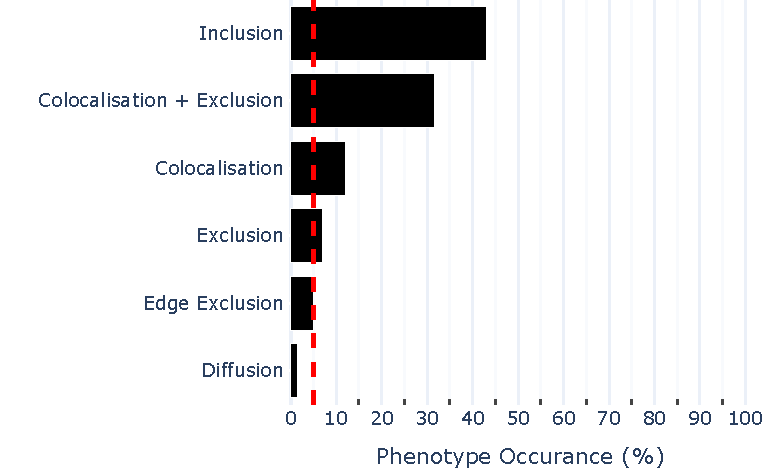
\includegraphics[width=1\linewidth]{10. Chapter 5/Figs/03. IFIT2-FLAG/03. IFIT2F/01. pIB/04. bar_bi2f_hnhp.pdf} 
    \end{subfigure}
    \begin{subfigure}{0.495\textwidth}
        \caption{}
        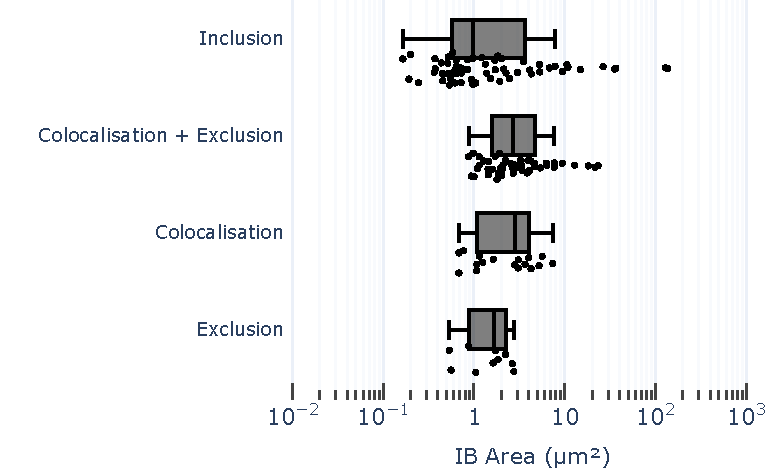
\includegraphics[width=1\linewidth]{10. Chapter 5/Figs/03. IFIT2-FLAG/03. IFIT2F/01. pIB/05. box_bi2f_hnhp.pdf}
    \end{subfigure}
    \caption[Observed Phenotypes of Exogenous Bovine IFIT2 in the Context of hRSV Pseudo Inclusion Bodies in VERO Cell Line, as Detected by FLAG Antibody.]{\textbf{Observed Phenotypes of Exogenous Bovine IFIT2 in the Context of hRSV Pseudo Inclusion Bodies in VERO Cell Line, as Detected by FLAG Antibody.} Vero cells were transfected with hRSV N and P, along with bovine IFIT2-FLAG containing plasmids using TransIT-X2 and were fixed after 24 hours. Cells were labeled with anti-RSV N and anti-FLAG antibodies and imaged on confocal microscope. Panel (a) shows percentual proportions of observed phenotypes between hRSV pseudo inclusion bodies and exogenous bovine IFIT2 (142 observations), with the red dotted line denoting the 5\% threshold, marking phenotypes considered relevant above this limit. Panel (b) shows the IB area in \(\mu m^2\) per observed relevant phenotype.}
    \label{fig:Observed Phenotypes of Exogenous Bovine IFIT2 in the Context of hRSV Pseudo Inclusion Bodies in VERO Cell Line, as Detected by FLAG Antibody}
\end{figure}

\begin{figure}
    \centering
    \includegraphics[width=1\linewidth]{10. Chapter 5/Figs/03. IFIT2-FLAG/03. IFIT2F/01. pIB/06. bi2f-hnhp.pdf}
    \caption[Representative Images of Observed Phenotypes of Exogenous Bovine IFIT2 in the Context of hRSV Pseudo Inclusion Bodies in VERO Cell Line, as Detected by FLAG Antibody.]{\textbf{Representative Images of Observed Phenotypes of Exogenous Bovine IFIT2 in the Context of hRSV Pseudo Inclusion Bodies in VERO Cell Line, as Detected by FLAG Antibody.} Vero cells were transfected with hRSV N and P, along with bovine IFIT2-FLAG containing plasmids using TransIT-X2 and were fixed after 24 hours. Cellular nuclei were stained with DAPI (yellow), and cells were double-labeled with anti-RSV N (cyan) and anti-FLAG (magenta) antibodies. This figure showcases representative examples of relevant phenotypes in the interaction between exogenous bovine IFIT2 and hRSV pseudo inclusion bodies. These phenotypes are presented in descending order based on their percentage proportions. The scale bar indicates 2 \(\mu m\).}
    \label{fig:Representative Images of Observed Phenotypes of Exogenous Bovine IFIT2 in the Context of hRSV Pseudo Inclusion Bodies in VERO Cell Line, as Detected by FLAG Antibody}
\end{figure}

\begin{figure}
    \begin{subfigure}{0.495\textwidth}
        \caption{}
        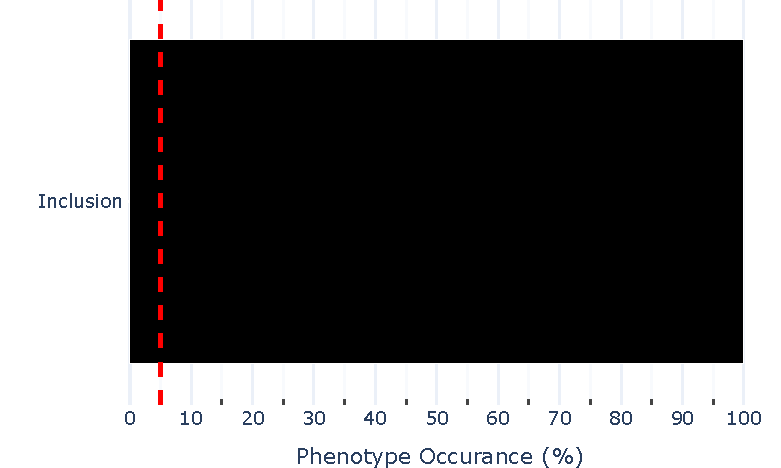
\includegraphics[width=1\linewidth]{10. Chapter 5/Figs/03. IFIT2-FLAG/03. IFIT2F/01. pIB/07. bar_bi2f_bnbp.pdf} 
    \end{subfigure}
    \begin{subfigure}{0.495\textwidth}
        \caption{}
        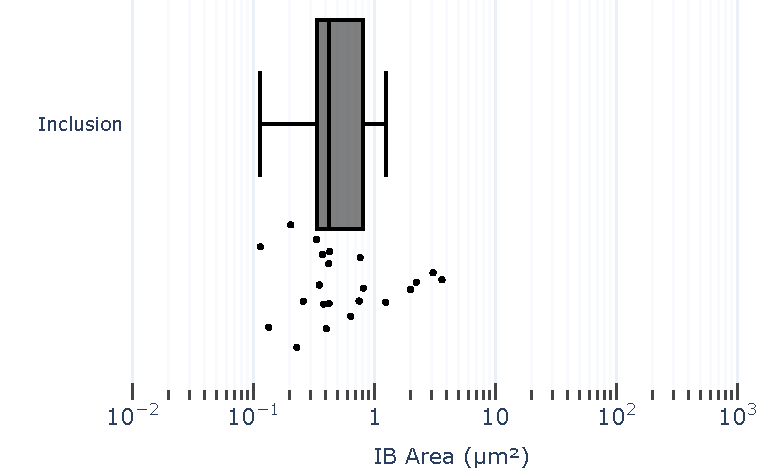
\includegraphics[width=1\linewidth]{10. Chapter 5/Figs/03. IFIT2-FLAG/03. IFIT2F/01. pIB/08. box_bi2f_bnbp.pdf}
    \end{subfigure}
    \caption[Observed Phenotypes of Exogenous Bovine IFIT2 in the Context of bRSV Pseudo Inclusion Bodies in VERO Cell Line, as Detected by FLAG Antibody.]{\textbf{Observed Phenotypes of Exogenous Bovine IFIT2 in the Context of bRSV Pseudo Inclusion Bodies in VERO Cell Line, as Detected by FLAG Antibody.} Vero cells were transfected with bRSV N and P, along with bovine IFIT2-FLAG containing plasmids using TransIT-X2 and were fixed after 24 hours. Cells were labeled with anti-RSV N and anti-FLAG antibodies and imaged on confocal microscope. Panel (a) shows percentual proportions of observed phenotypes between bRSV pseudo inclusion bodies and exogenous bovine IFIT2 (22 observations), with the red dotted line denoting the 5\% threshold, marking phenotypes considered relevant above this limit. Panel (b) shows the IB area in \(\mu m^2\) per observed relevant phenotype.}
    \label{fig:Observed Phenotypes of Exogenous Bovine IFIT2 in the Context of bRSV Pseudo Inclusion Bodies in VERO Cell Line, as Detected by FLAG Antibody}
\end{figure}

\begin{figure}
    \centering
    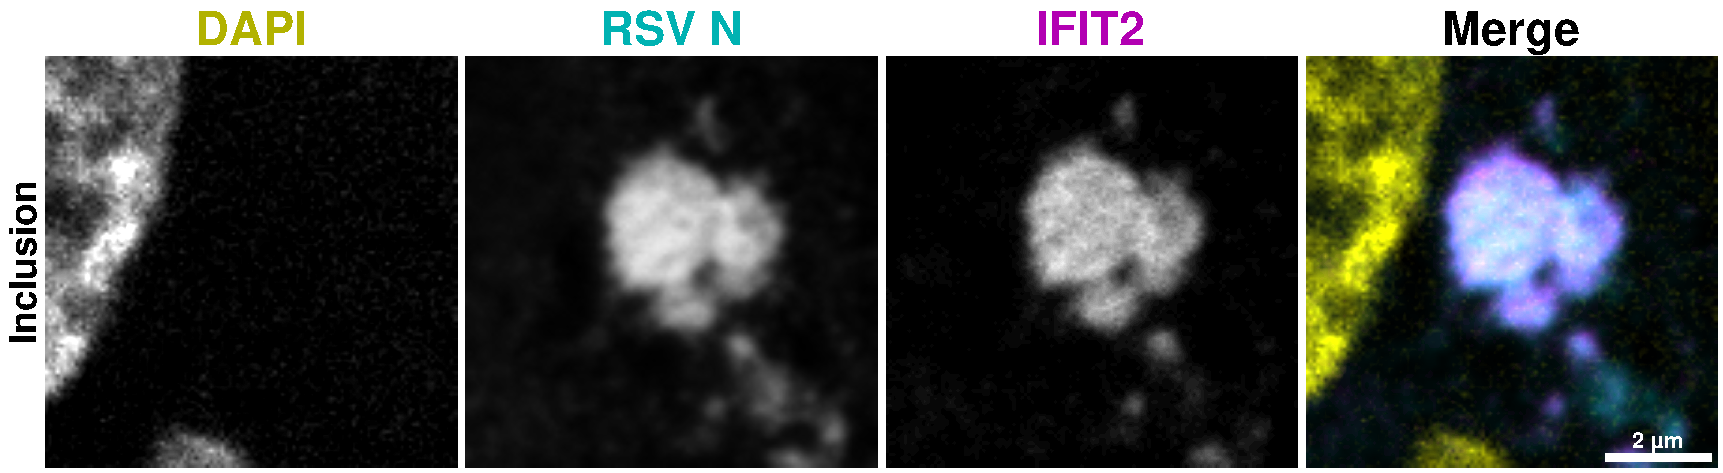
\includegraphics[width=1\linewidth]{10. Chapter 5/Figs/03. IFIT2-FLAG/03. IFIT2F/01. pIB/09. bi2f-bnbp.pdf}
    \caption[Representative Images of Observed Phenotypes of Exogenous Bovine IFIT2 in the Context of bRSV Pseudo Inclusion Bodies in VERO Cell Line, as Detected by FLAG Antibody.]{\textbf{Representative Images of Observed Phenotypes of Exogenous Bovine IFIT2 in the Context of bRSV Pseudo Inclusion Bodies in VERO Cell Line, as Detected by FLAG Antibody.} Vero cells were transfected with bRSV N and P, along with bovine IFIT2-FLAG containing plasmids using TransIT-X2 and were fixed after 24 hours. Cellular nuclei were stained with DAPI (yellow), and cells were double-labeled with anti-RSV N (cyan) and anti-FLAG (magenta) antibodies. This figure showcases representative examples of relevant phenotypes in the interaction between exogenous bovine IFIT2 and bRSV pseudo inclusion bodies. These phenotypes are presented in descending order based on their percentage proportions. The scale bar indicates 2 \(\mu m\).}
    \label{fig:Representative Images of Observed Phenotypes of Exogenous Bovine IFIT2 in the Context of bRSV Pseudo Inclusion Bodies in VERO Cell Line, as Detected by FLAG Antibody}
\end{figure}

\subsubsection{Exogenous IFIT2-FLAG During RSV Infection} \label{Exogenous IFIT2-FLAG During RSV Infection}
Overexpressed human IFIT2 during hRSV infection shows several phenotypes (in this experiment). We see IFIT2 being excluded from the IB interior while being concentrated to the IB ring (top panel); IFIT2 forming concentrated inclusion inside the IB structure (2nd panel); IFIT2 being excluded from the IB interior but colocalising to the IB ring and forming spots inside of the IB (3rd panel); and IFIT2 being diffused evenly through the cytoplasm and the IB structure (last panel). The different phenotypes suggest that IBs are dynamic structures, and the localisation depends on factors we do not comprehend yet. 

\begin{figure}
    \begin{subfigure}{0.495\textwidth}
        \caption{}
        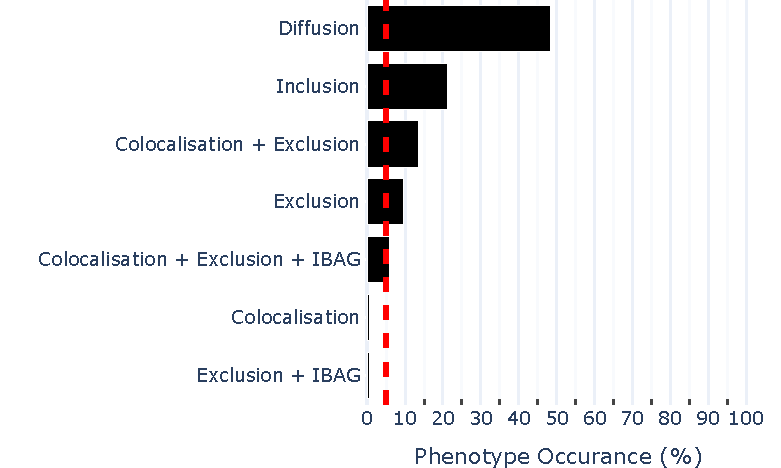
\includegraphics[width=1\linewidth]{10. Chapter 5/Figs/03. IFIT2-FLAG/03. IFIT2F/02. Infection Transfection/01. bar_hi2f_hrsv.pdf} 
    \end{subfigure}
    \begin{subfigure}{0.495\textwidth}
        \caption{}
        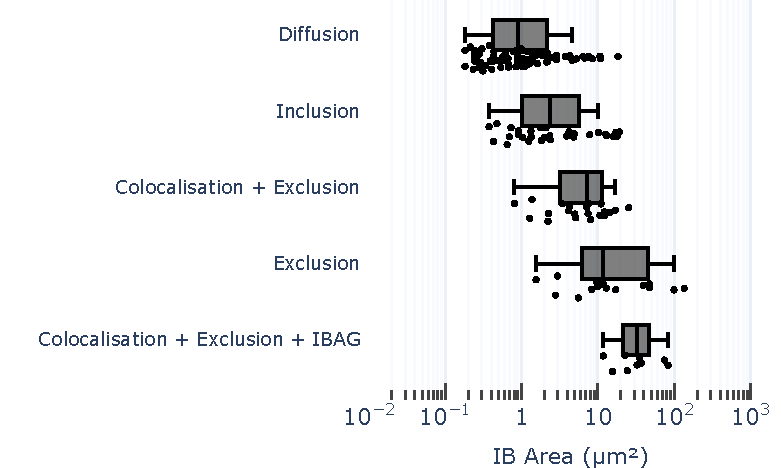
\includegraphics[width=1\linewidth]{10. Chapter 5/Figs/03. IFIT2-FLAG/03. IFIT2F/02. Infection Transfection/02. box_hi2f_hrsv.pdf}
    \end{subfigure}
    \caption[Observed Phenotypes of Exogenous hIFIT2 in the Context of hRSV Inclusion Bodies in VERO Cell Line.]{\textbf{Observed Phenotypes of Exogenous hIFIT2 in the Context of hRSV Inclusion Bodies in VERO Cell Line.} Vero cells were infected with human RSV at MOI 1. 24 HPI, the cells were transfected with hIFIT2-FLAG containing plasmids using TransIT-X2 and were fixed after further 24 hours. Cells were labeled with anti-RSV N and anti-FLAG antibodies and imaged on confocal microscope. Panel (a) shows percentual proportions of observed phenotypes between hRSV inclusion bodies and exogenous hIFIT2 (155 observations), with the red dotted line denoting the 5\% threshold, marking phenotypes considered relevant above this limit. Panel (b) shows the IB area in \(\mu m^2\) per observed relevant phenotype.}
    \label{fig:Observed Phenotypes of Exogenous hIFIT2 in the Context of hRSV Inclusion Bodies in VERO Cell Line}
\end{figure}

\begin{figure}
    \centering
    \includegraphics[width=1\linewidth]{10. Chapter 5/Figs/03. IFIT2-FLAG/03. IFIT2F/02. Infection Transfection/03. hi2f-hrsv.pdf}
    \caption[Representative Images of Observed Phenotypes of Exogenous hIFIT2 in the Context of hRSV Inclusion Bodies in VERO Cell Line.]{\textbf{Representative Images of Observed Phenotypes of Exogenous hIFIT2 in the Context of hRSV Inclusion Bodies in VERO Cell Line.} Vero cells were infected with human RSV at MOI 1. 24 HPI, the cells were transfected with hIFIT2-FLAG containing plasmids using TransIT-X2 and were fixed after further 24 hours. Cellular nuclei were stained with DAPI (yellow), and cells were double-labeled with anti-RSV N (cyan) and anti-FLAG (magenta) antibodies. This figure showcases representative examples of relevant phenotypes in the interaction between exogenous hIFIT2 and hRSV inclusion bodies. These phenotypes are presented in descending order based on their percentage proportions. The scale bar indicates 2 \(\mu m\).}
    \label{fig:Representative Images of Observed Phenotypes of Exogenous hIFIT2 in the Context of hRSV Inclusion Bodies in VERO Cell Line}
\end{figure}

In the follow up experiment, exogenous bovine IFIT2 in the context of human RSV infection shows the same two phenotypes. It is either excluded from the IBs (middle panel) or colocalises with the ring structure of the IBs (top and bottom panel; highlighted with arrows).

\begin{figure}
    \begin{subfigure}{0.495\textwidth}
        \caption{}
        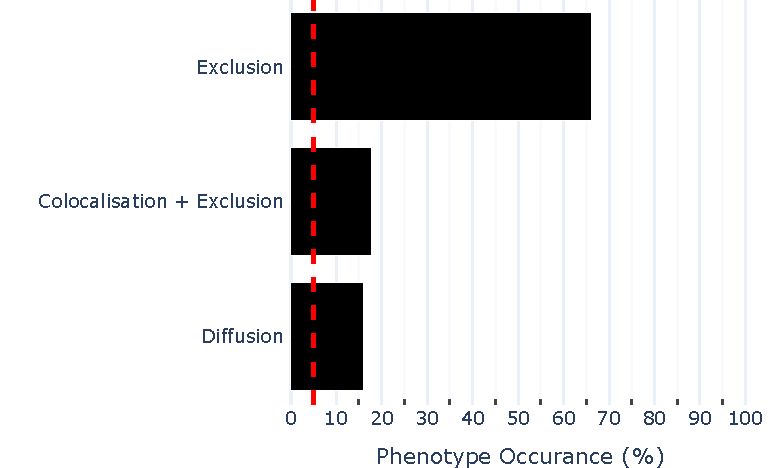
\includegraphics[width=1\linewidth]{10. Chapter 5/Figs/03. IFIT2-FLAG/03. IFIT2F/02. Infection Transfection/04. bar_bi2f_hrsv.pdf} 
    \end{subfigure}
    \begin{subfigure}{0.495\textwidth}
        \caption{}
        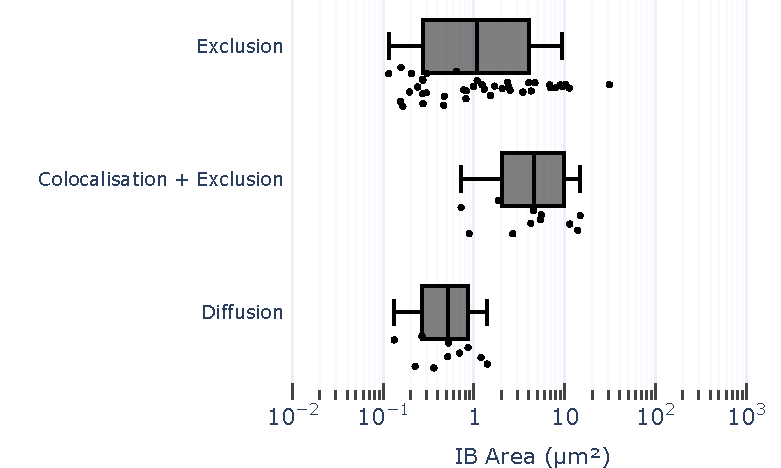
\includegraphics[width=1\linewidth]{10. Chapter 5/Figs/03. IFIT2-FLAG/03. IFIT2F/02. Infection Transfection/05. box_bi2f_hrsv.pdf}
    \end{subfigure}
    \caption[Observed Phenotypes of Exogenous bIFIT2 in the Context of hRSV Inclusion Bodies in VERO Cell Line.]{\textbf{Observed Phenotypes of Exogenous bIFIT2 in the Context of hRSV Inclusion Bodies in VERO Cell Line.} Vero cells were infected with human RSV at MOI 1. 24 HPI, the cells were transfected with bIFIT2-FLAG containing plasmids using TransIT-X2 and were fixed after further 24 hours. Cells were labeled with anti-RSV N and anti-FLAG antibodies and imaged on confocal microscope. Panel (a) shows percentual proportions of observed phenotypes between hRSV inclusion bodies and exogenous bIFIT2 (62 observations), with the red dotted line denoting the 5\% threshold, marking phenotypes considered relevant above this limit. Panel (b) shows the IB area in \(\mu m^2\) per observed relevant phenotype.}
    \label{fig:Observed Phenotypes of Exogenous bIFIT2 in the Context of hRSV Inclusion Bodies in VERO Cell Line}
\end{figure}

\begin{figure}
    \centering
    \includegraphics[width=1\linewidth]{10. Chapter 5/Figs/03. IFIT2-FLAG/03. IFIT2F/02. Infection Transfection/06. bi2f-hrsv.pdf}
    \caption[Representative Images of Observed Phenotypes of Exogenous bIFIT2 in the Context of hRSV Inclusion Bodies in VERO Cell Line.]{\textbf{Representative Images of Observed Phenotypes of Exogenous bIFIT2 in the Context of hRSV Inclusion Bodies in VERO Cell Line.} Vero cells were infected with human RSV at MOI 1. 24 HPI, the cells were transfected with bIFIT2-FLAG containing plasmids using TransIT-X2 and were fixed after further 24 hours. Cellular nuclei were stained with DAPI (yellow), and cells were double-labeled with anti-RSV N (cyan) and anti-FLAG (magenta) antibodies. This figure showcases representative examples of relevant phenotypes in the interaction between exogenous bIFIT2 and hRSV inclusion bodies. These phenotypes are presented in descending order based on their percentage proportions. The scale bar indicates 2 \(\mu m\).}
    \label{fig:Representative Images of Observed Phenotypes of Exogenous bIFIT2 in the Context of hRSV Inclusion Bodies in VERO Cell Line}
\end{figure}

Exogenous bovine IFIT2 during bovine RSV infection seems to be excluded from the inclusion bodies, although the data is not great and the IFIT2 is aggregated in both cells shown.

\begin{figure}
    \begin{subfigure}{0.495\textwidth}
        \caption{}
        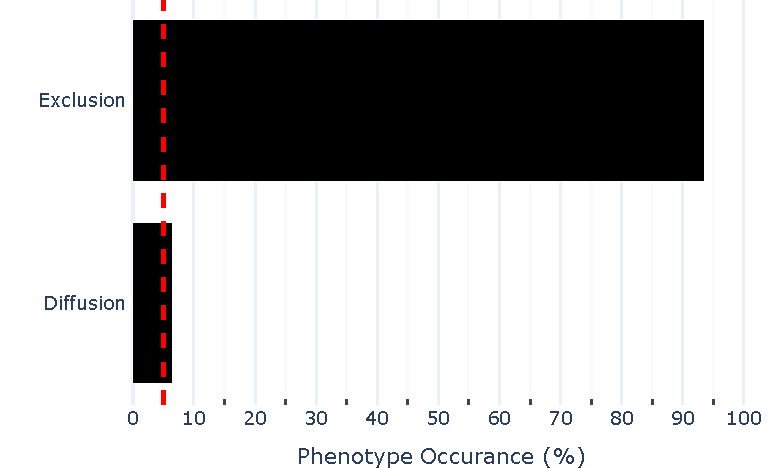
\includegraphics[width=1\linewidth]{10. Chapter 5/Figs/03. IFIT2-FLAG/03. IFIT2F/02. Infection Transfection/07. bar_bi2f_brsv.pdf} 
    \end{subfigure}
    \begin{subfigure}{0.495\textwidth}
        \caption{}
        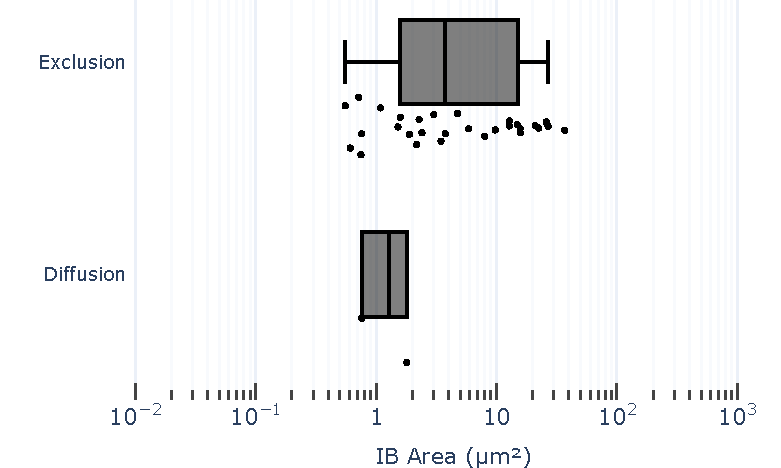
\includegraphics[width=1\linewidth]{10. Chapter 5/Figs/03. IFIT2-FLAG/03. IFIT2F/02. Infection Transfection/08. box_bi2f_brsv.pdf}
    \end{subfigure}
    \caption[Observed Phenotypes of Exogenous bIFIT2 in the Context of bRSV Inclusion Bodies in VERO Cell Line.]{\textbf{Observed Phenotypes of Exogenous bIFIT2 in the Context of bRSV Inclusion Bodies in VERO Cell Line.} Vero cells were infected with human RSV at MOI 1. 24 HPI, the cells were transfected with bIFIT2-FLAG containing plasmids using TransIT-X2 and were fixed after further 24 hours. Cells were labeled with anti-RSV N and anti-FLAG antibodies and imaged on confocal microscope. Panel (a) shows percentual proportions of observed phenotypes between bRSV inclusion bodies and exogenous bIFIT2 (31 observations), with the red dotted line denoting the 5\% threshold, marking phenotypes considered relevant above this limit. Panel (b) shows the IB area in \(\mu m^2\) per observed relevant phenotype.}
    \label{fig:Observed Phenotypes of Exogenous bIFIT2 in the Context of bRSV Inclusion Bodies in VERO Cell Line}
\end{figure}

\begin{figure}
    \centering
    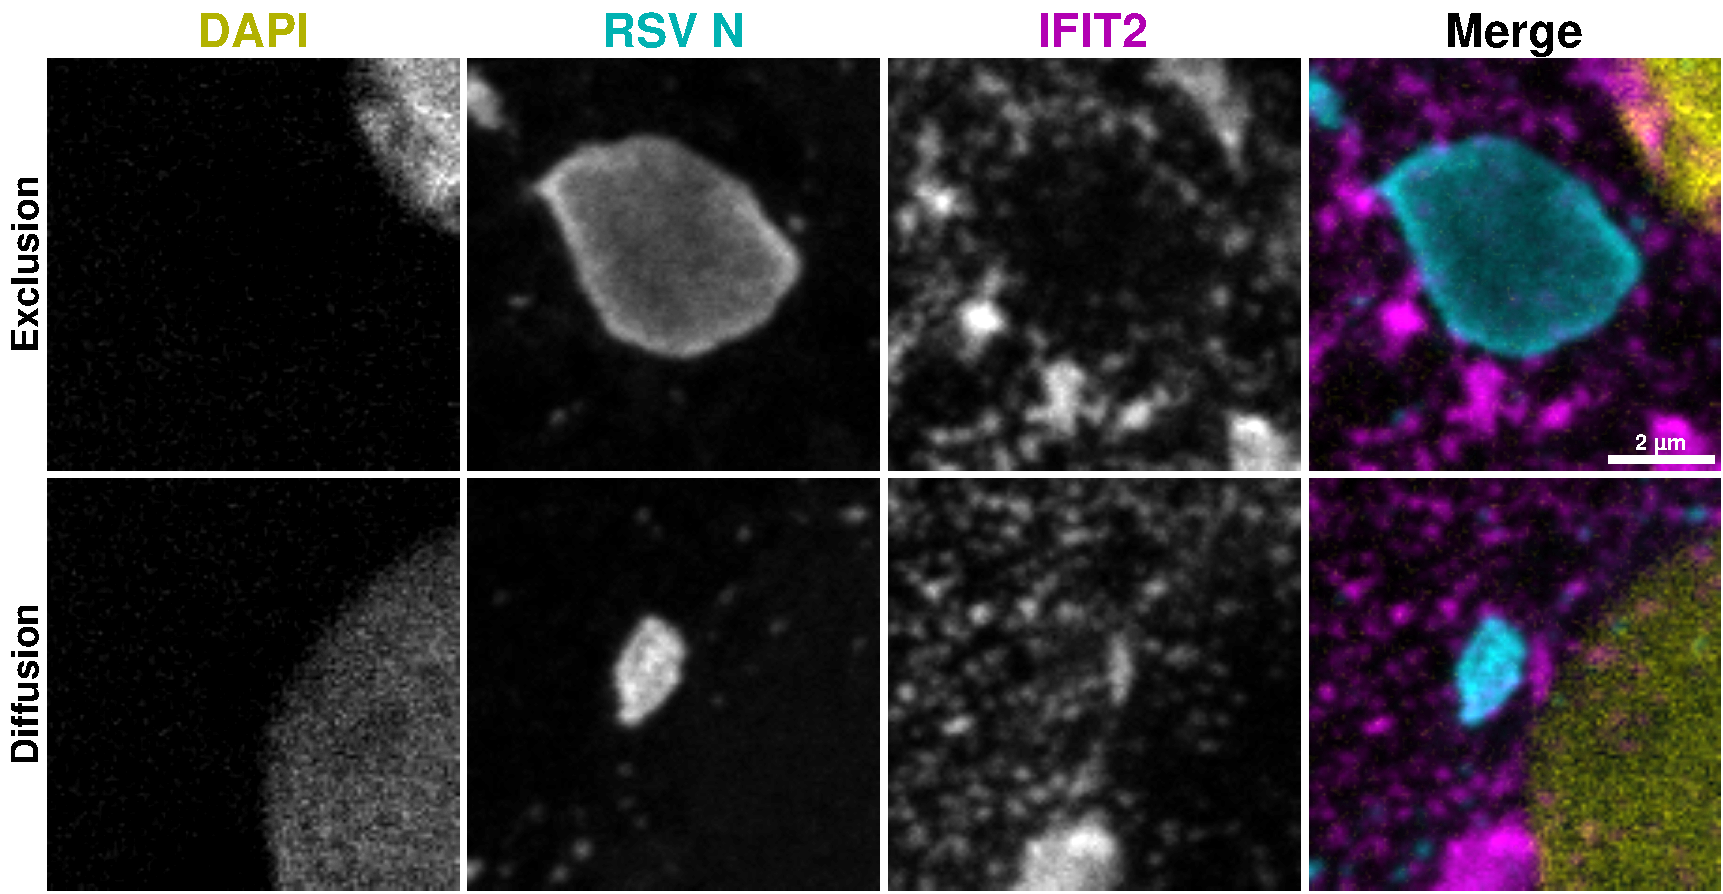
\includegraphics[width=1\linewidth]{10. Chapter 5/Figs/03. IFIT2-FLAG/03. IFIT2F/02. Infection Transfection/09. bi2f-brsv.pdf}
    \caption[Representative Images of Observed Phenotypes of Exogenous bIFIT2 in the Context of bRSV Inclusion Bodies in VERO Cell Line.]{\textbf{Representative Images of Observed Phenotypes of Exogenous bIFIT2 in the Context of bRSV Inclusion Bodies in VERO Cell Line.} Vero cells were infected with human RSV at MOI 1. 24 HPI, the cells were transfected with bIFIT2-FLAG containing plasmids using TransIT-X2 and were fixed after further 24 hours. Cellular nuclei were stained with DAPI (yellow), and cells were double-labeled with anti-RSV N (cyan) and anti-FLAG (magenta) antibodies. This figure showcases representative examples of relevant phenotypes in the interaction between exogenous bIFIT2 and bRSV inclusion bodies. These phenotypes are presented in descending order based on their percentage proportions. The scale bar indicates 2 \(\mu m\).}
    \label{fig:Representative Images of Observed Phenotypes of Exogenous bIFIT2 in the Context of bRSV Inclusion Bodies in VERO Cell Line}
\end{figure}

\subsubsection{Summary} \label{Summary-i2-flag}
Overexpressing human IFIT2-FLAG does not seem to be detrimental to the cells. Exogenous human IFIT2 seems to form inclusions inside human pIB structures. It also colocalises with the pIB associated filamentous network. This data is consistent with IFIT2A antibody staining. IFIT2B staining showed inclusion inside pIB but failed to show the colocalization with the filamentous network. Exogenous bovine IFIT2 colocalises to the edge of human pIBs, which is in contrast to what we see with endogenous and exogenous human IFIT2 and its interaction with human pIBs. Exogenous human IFIT2 during human RSV infection showed different phenotypes in 2 different experiments. In the first experiment we observed it to: form inclusions inside the IB structure; be excluded from IB but colocalise to the IB ring; be excluded from the IB but colocalise to the ring and have spots inside the IB structure; or to be diffused through cytoplasm and IB equally. In the second experiment we observed it to be either completely excluded from the IBs or to colocalise with them. Exogenous bovine IFIT2 during human RSV infection was either completely excluded from the IB or was colocalised to the ring of the structure. This was consistently seen in both experiments conducted. Exogenous bovine IFIT2 during bovine RSV infection seems to be excluded from the IBs.
\subsection{The Impact of RNA-Binding on IFIT2-pIB Interaction} \label{subsec:The Impact of RNA-Binding on IFIT2-pIB Interaction}
\subsubsection{The Generation of Bovine IFIT2 RNA-Binding Mutant} \label{The Generation of Bovine IFIT2 RNA-Binding Mutant}
Using published data about hIFIT2 rna-binding mutant

Difficulty of using alpha-fold with IFIT2 due to the swap domain

Using SWISS-MODEL to predict bIFIT2 structure from published hIFIT2 structures

Alignment of both structures, assessment of electrostatic charges and establishment of residues to be mutated

Primer design and mutagenesis procedure based on published hIFIT2 RNA-binding mutant paper

\begin{figure}
    \centering
    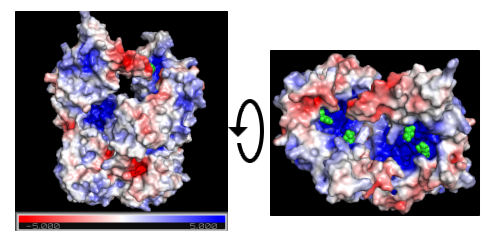
\includegraphics[width=1\linewidth]{10. Chapter 5/Figs/05. IFIT2-RNA binding mutant/01. structure.png}
    \caption[ifit2 mutant structure]{ifit2 mutant structure}
    \label{fig:ifit2 mutant structure}
\end{figure}

%i2f-24
%bi2f24
Cell Line: VERO
Treatment: bIFIT2-FLAG-RBM
Detecting magenta: exogenous bovine IFIT2 RBM
Detecting cyan: background

Exogenous bovine IFIT2 RNA-binding mutant (RBM) seems to have the same distribution and effect on the cell as human IFIT2-FLAG overexpression.

\begin{figure}
    \centering
    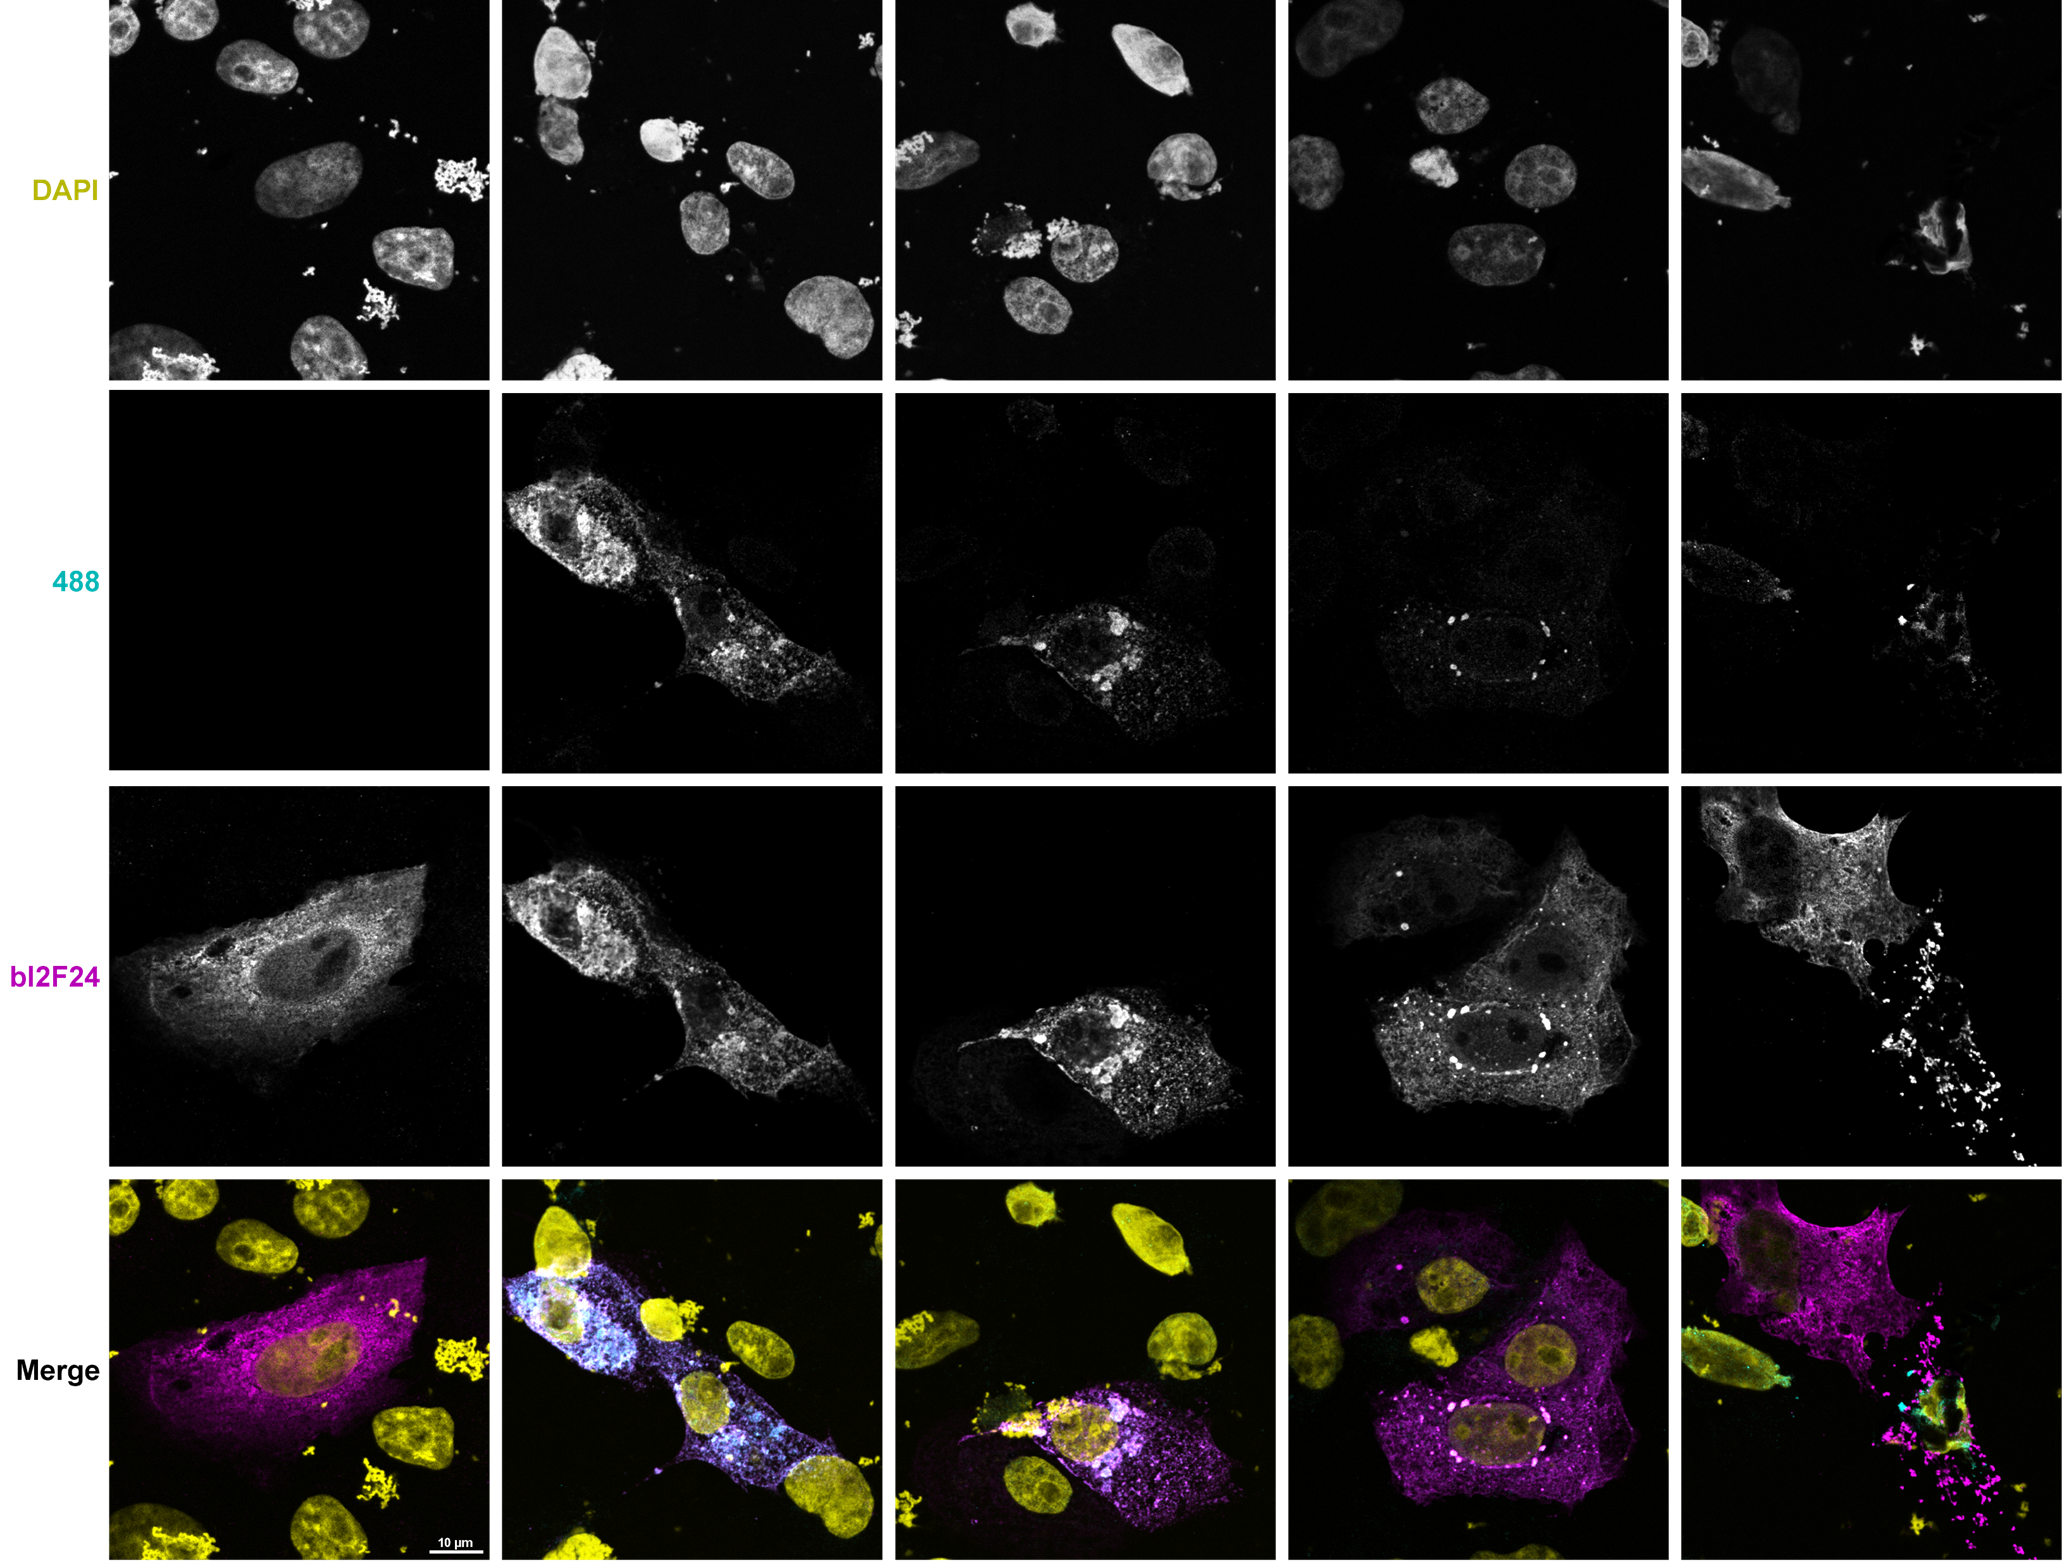
\includegraphics[width=1\linewidth]{10. Chapter 5/Figs/05. IFIT2-RNA binding mutant/02. bi2f24.png}
    \caption[bi2f24]{bi2f24}
    \label{fig:bi2f24}
\end{figure}

\subsubsection{Bovine IFIT2 RNA-Binding Mutant and RSV pIBs} \label{Bovine IFIT2 RNA-Binding Mutant and RSV pIBs}
%bi2f24 + hnhp
Cell Line: VERO
Treatment: hNhP + bIFIT2-FLAG-RBM
Detecting magenta: exogenous bovine IFIT2 RBM
Detecting cyan: human pIB

In the second experiment we see consistent colocalization and/or inclusion of bovine IFIT2 RNA-binding mutant with human pseudo inclusion bodies.

\begin{figure}
    \centering
    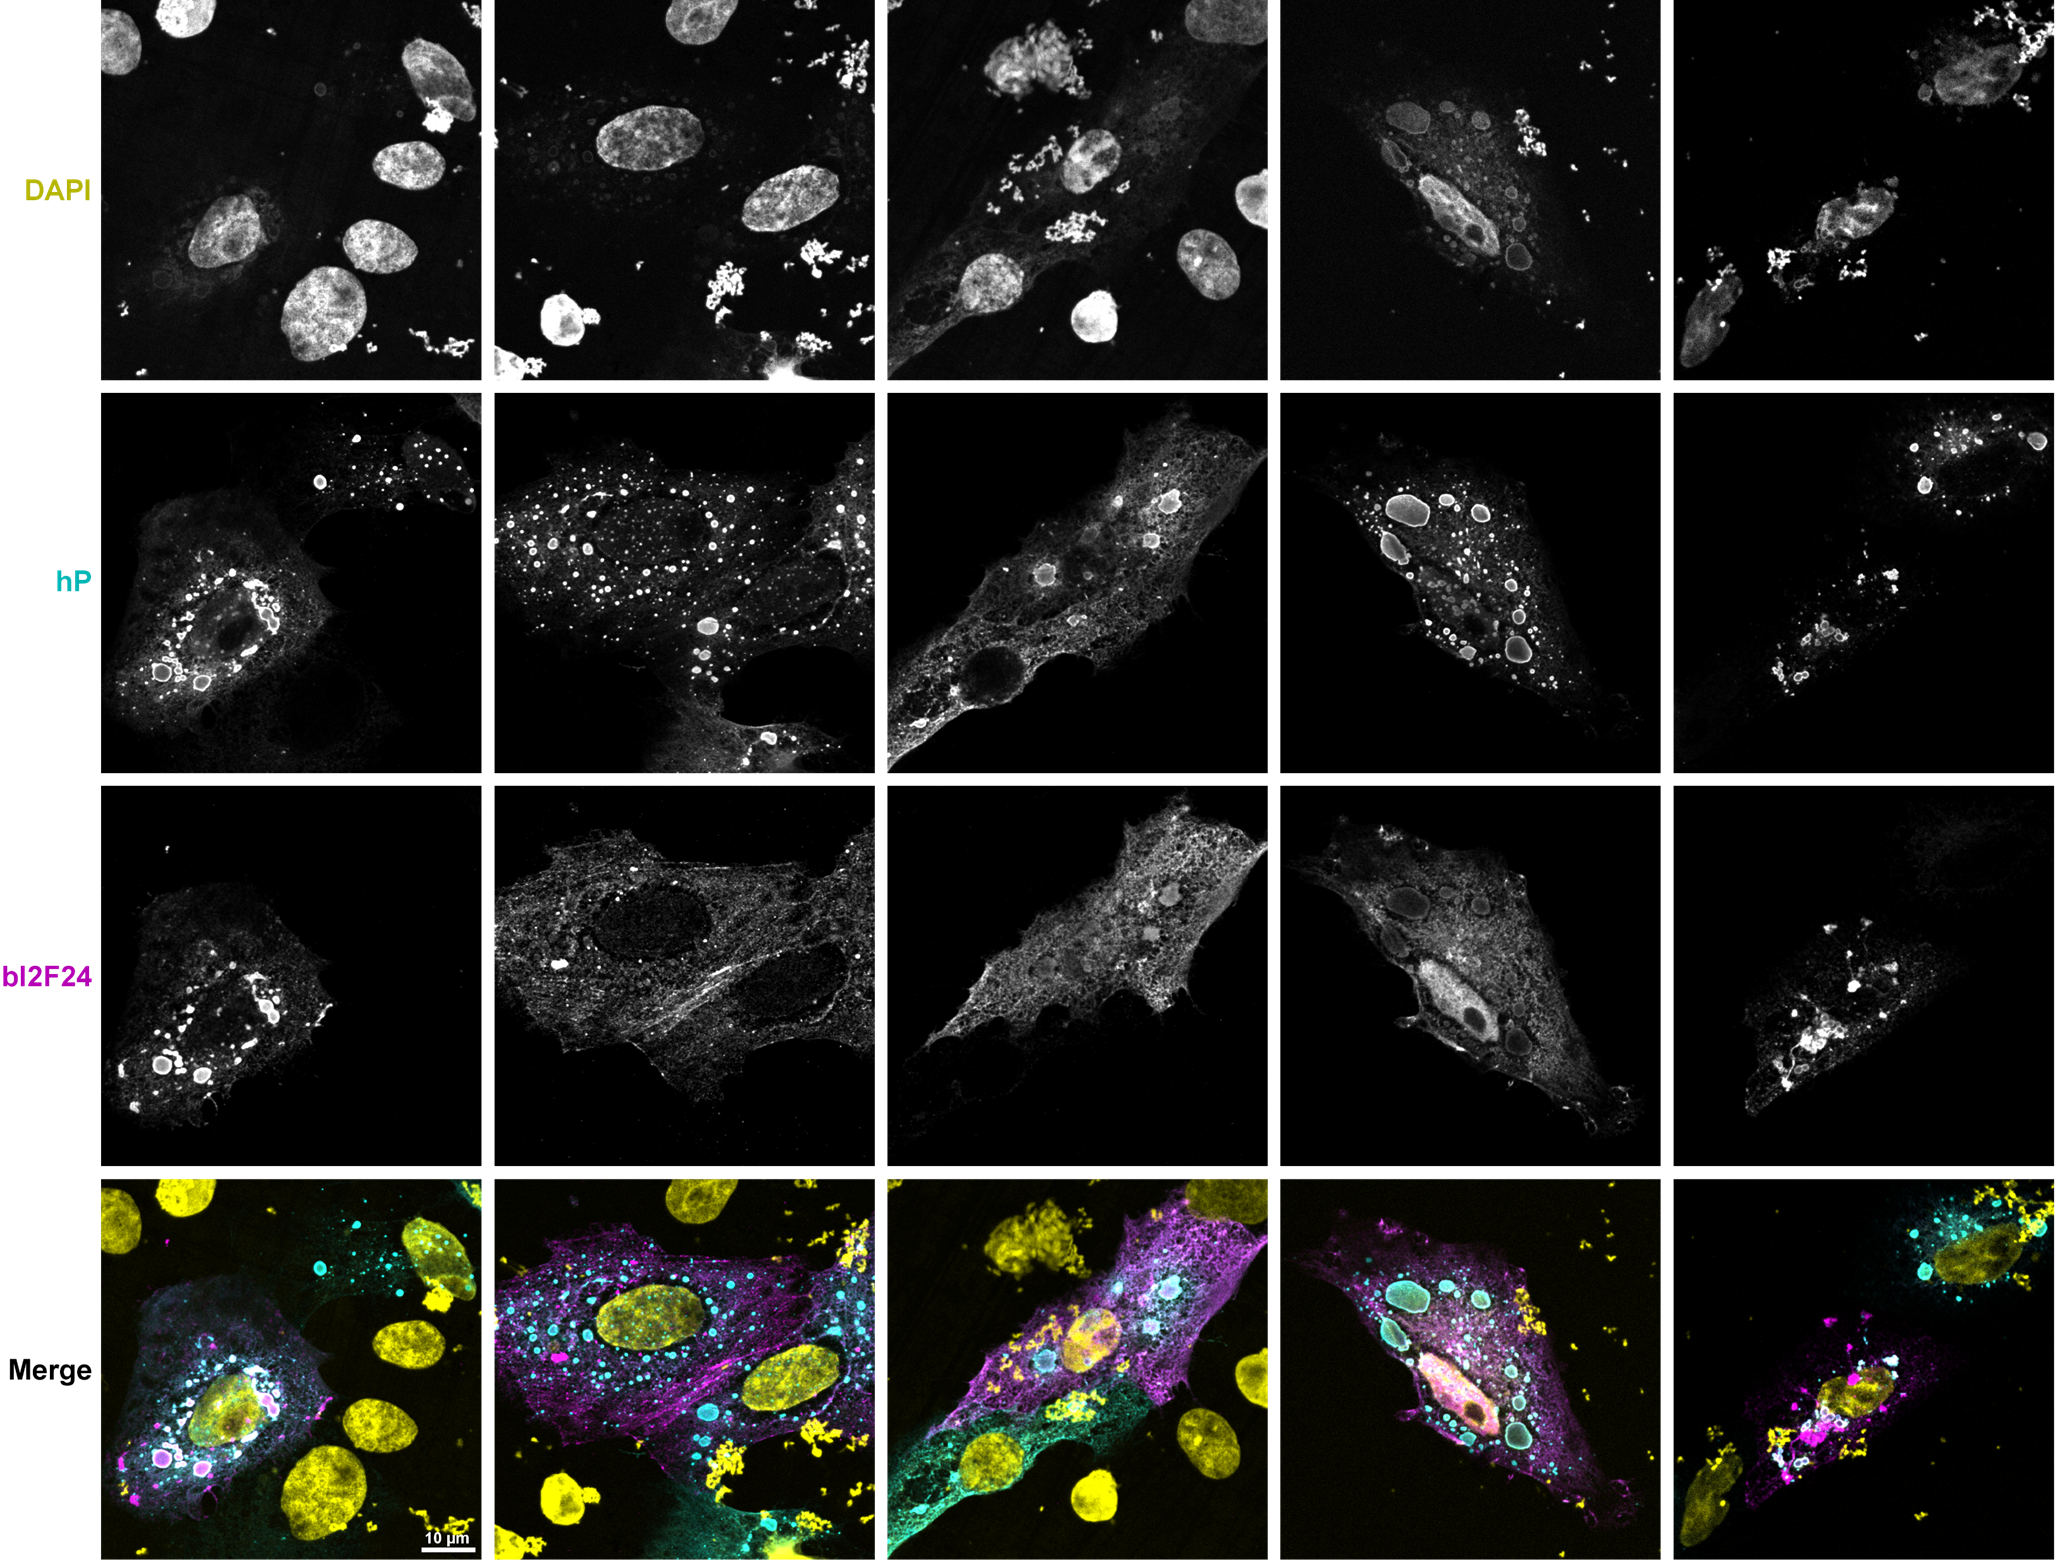
\includegraphics[width=0.5\linewidth]{10. Chapter 5/Figs/05. IFIT2-RNA binding mutant/03. bi2f hnhp.png}
    \caption[bi2f24 + hnhp]{bi2f24 + hnhp}
    \label{fig:bi2f24 + hnhp}
\end{figure}

\subsubsection{Summary}
We have described how bovine IFIT2 RNA-binding mutant was designed based on the published human IFIT2 RNA-binding mutant data (needs to be annotated more). Overexpression of bovine IFIT2 RNA-binding mutant yields cellular distribution and morphology similar to what was observed with overexpressing human IFIT2-FLAG, suggesting that the mutant proteins are not toxic to the cells. In the first experiment where we were looking at interaction between bovine IFIT2 RNA-binding mutant and human pseudo inclusion bodies we saw several phenotypes. We observed bovine IFIT2 RNA-binding mutant being excluded from small and big pIBs and pIB associated filamentous network, while fully or partially colocalising with other pIBs. In a subsequent experiment we observed only colocalization and inclusion formation. When assessing the interaction between bovine IFIT2 RNA-binding mutant and human pIBs formed using wild-type human RSV P and GFP-tagged human RSV N, we observed consistently in two experiments that bovine IFIT2 RNA-binding mutant colocalises to the pIB structures.

\subsection{Liquid-Liquid Phase Separation Analysis} \label{subsec:Liquid-Liquid Phase Separation Analysis}
Add stuff about likelihood of IFIT and viral proteins and their propensity to phase separate \newline
This is using a online tool called PSPredictor


\section{Discussion} \label{sec:Discussion-Chapter5}
transfecting bi2f24 + bngfp + p inhibits bpIBs
\subsection{Discrepancy Between IFIT2 A and B Antibodies} \label{subsec:Discrepancy Between IFIT2 A and B Antibodies}
%Discussion About Differences Seen Between the Two Antibodies in Previous Subchapter
IFIT2A shows monkey IFIT2 forming inclusion within the pIB structure, while also colocalising with the pIB-associated filamentous network.  IFIT2B shows exclusion from both pIB and the filaments.

IFIT2A shows overexpressed hIFIT2-FLAG to form inclusion inside the pIBs and colocalization with the filamentous network. IFIT2B also shows inclusion inside the pIBs but shows potential exclusion from the filamentous network.
IFIT2A shows colocalization to the ring and inner edge of human IBs with occasional inclusions. IFIT2B shows complete and partial exclusion from the human IB structures. 

IFT2A shows bovine IFIT2 col9ocalisation to the with the ring structure of bovine IBs. IFIT2B shows partial exclusion; exclusion from the IB ring and inner edge with IBAG-like inclusions; and diffusion through the IB structure.
%Differences Between the Two Antibodies Other Than IB Staining
%Human Protein Atlas Show Cytoplasmic Localisation Similar to IFIT2B

\begin{figure}
    \centering
    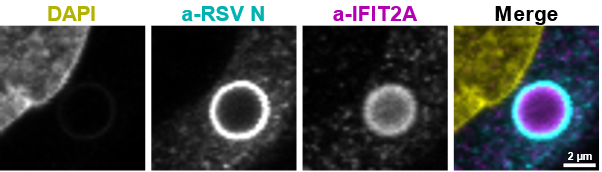
\includegraphics[width=1\linewidth]{10. Chapter 5//Figs//01. I2A/04. i2a a549 hrsv n.png}
    \caption[example ifi2a hrsv]{example ifi2a hrsv}
    \label{fig:example ifi2a hrsv}
\end{figure}

IFIT2A antibody shows mainly cytoplasmic distribution (although some spots are visible)


\begin{figure}
    \centering
    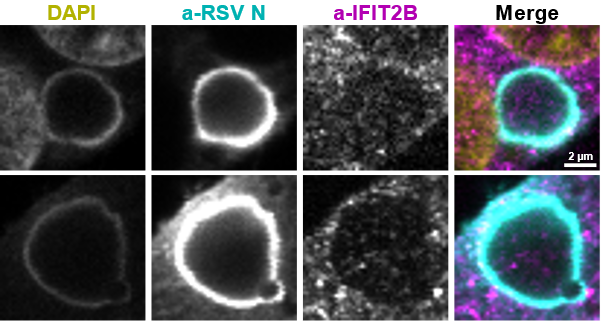
\includegraphics[width=1\linewidth]{10. Chapter 5//Figs//02. I2B/03. i2b a549 hrsv n.png}
    \caption[example ifi2b hrsv]{example ifi2b hrsv}
    \label{fig:example ifi2b hrsv}
\end{figure}

IFIT2B shows mainly granular/vesicular distribution.

\begin{figure}
    \centering
    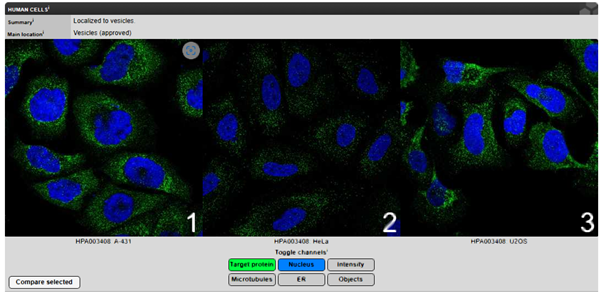
\includegraphics[width=1\linewidth]{10. Chapter 5//Figs//04. IFIT2AB Discussion/02. human protein atlas ifit2.png}
    \caption[human protein atlas ifit2]{human protein atlas ifit2}
    \label{fig:human protein atlas ifit2}
\end{figure}

Human protein atlas shows vesicular distribution of IFIT2.
Side note: second figure from section 1.1.1.2.3 shows cytoplasmic staining (like IFIT2A, but kinetochore microtubule staining (like IFIT2B).

%P Transfection Induces IFIT2A Signal but not IFIT2B Signal
Cell Line: 293T \newline
Treatment: hN and/or hP (EV – empty vector) \newline
Detecting magenta: endogenous human IFIT2 (A) \newline
Detecting cyan: N and/or P \newline

IFIT2 induction detected in hP and hP + hN conditions, suggesting that transfection of P induces IFIT2 expression (but this does not happen with IFIT1 or IFIT3 in the same cells).
About the different genomic regulation landscape… why does IFIT2 get induced but not other IFITs (within human genome which is well annotated)? 
Side note: No kinetochore microtubule staining (especially in first panel)

\begin{figure}
    \centering
    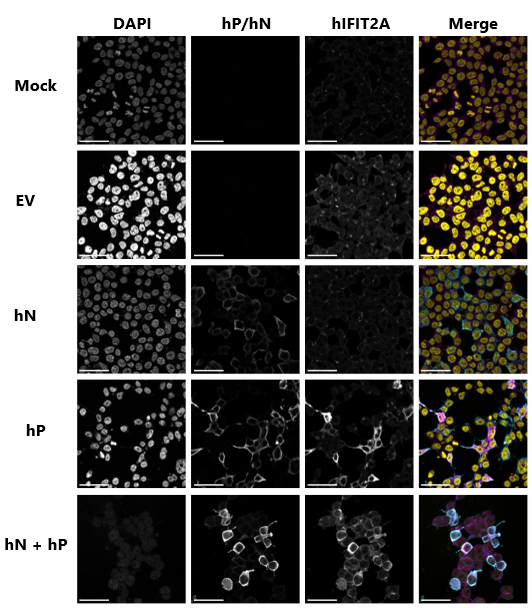
\includegraphics[width=1\linewidth]{10. Chapter 5//Figs//04. IFIT2AB Discussion/03. ifit2a p transfection.png}
    \caption[ifit2a p transfection]{ifit2a p transfection}
    \label{fig:ifit2a p transfection}
\end{figure}

Cell Line: 293T \newline
Treatment: hN and/or hP (EV – empty vector) \newline
Detecting magenta: endogenous human IFIT2 (B) \newline
Detecting cyan: N and/or P \newline

No detected IFIT2 induction in any of the conditions.
Side note: We can see kinetochore microtubule staining, especially in the first row.

\begin{figure}
    \centering
    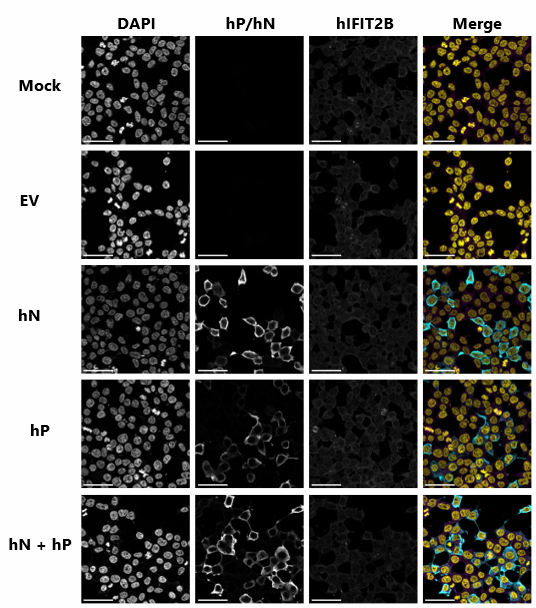
\includegraphics[width=1\linewidth]{10. Chapter 5//Figs//04. IFIT2AB Discussion/04. ifit2b p transfection.png}
    \caption[ifit2b p transfection]{ifit2b p transfection}
    \label{fig:ifit2b p transfection}
\end{figure}

%IFIT2B but not IFIT2A Stains Kinetochore Microtubules
Cell Line: MDBK \newline
Treatment: bRSV + bIFNa \newline
Detecting magenta: endogenous human IFIT2 (B) \newline
Detecting cyan: bovine IBs \newline

IFIT2B antibody consistently stains kinetochore microtubules in all cells regardless of the condition. This was figure that I had done already which had the kinetochore microtubule staining present, hence I included it here. I found only one minor paper about IFIT2 localisation that shows the same staining. Literature search looking at kinetochore proteomes never mentioned IFIT2, neither papers about anaphase/metaphase proteome.

\begin{figure}
    \centering
    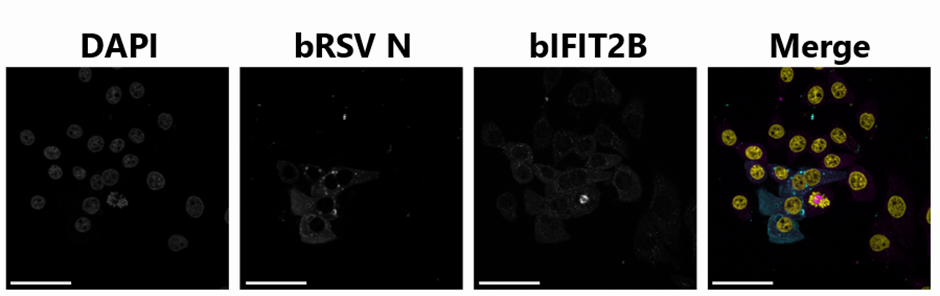
\includegraphics[width=1\linewidth]{10. Chapter 5//Figs//04. IFIT2AB Discussion/05. kinetochores.png}
    \caption[kinetochores]{kinetochores}
    \label{fig:kinetochores}
\end{figure}

This is figure from the paper that mentions mouse IFIT2 (GARG39) to be associated with microtubules during the different phases of cell cycle.
Side note: The IFIT2 distribution is cytoplasmic and not vesicular, like human protein atlas suggests.

\begin{figure}
    \centering
    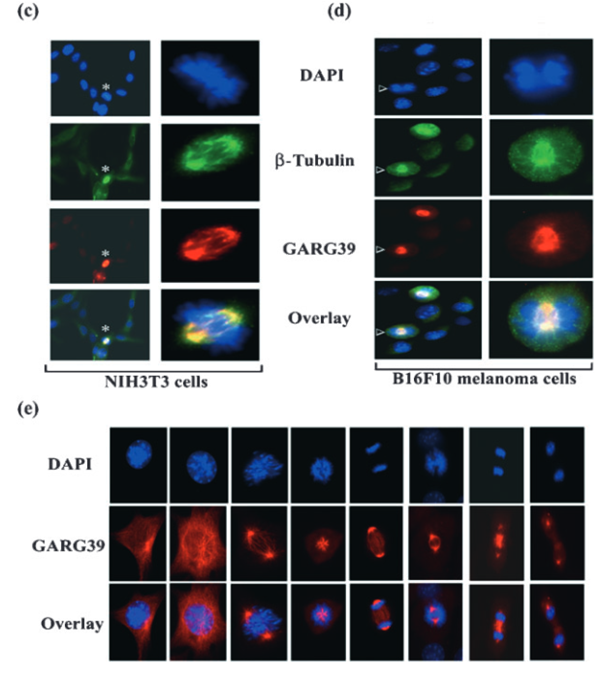
\includegraphics[width=1\linewidth]{10. Chapter 5//Figs//04. IFIT2AB Discussion/06. kinetochore published figure.png}
    \caption[kinetochore published figure]{kinetochore published figure}
    \label{fig:kinetochore published figure}
\end{figure}

%WB antibody validation
Western blots below are a validation of IFIT antibodies cross-reactivity. They are 293T cells transfected with empty vector or highlighted IFITs.

We see less material to be present in bovine samples, especially bovine IFIT3 sample.

IFIT2A antibody detects overexpressed human and bovine IFIT2, while also detecting overexpressed human and bovine IFIT3. We see differential staining between IFIT2A and IFIT3 antibody, hence we can conclude that IFIT2A is not detecting IFIT3 in IF analyses. IFIT2A is also detecting a moiety at 25 kDa, which we do not know the origin of (cellular sources as it is present in empty vector as well).

IFIT2B antibody detects human IFIT2. It fails to detect bovine IFIT2, however, this could be due to lower reactivity with the bovine IFIT2 and/or lower expression levels in that sample. Unlike in IFIT2A antibody, we see no reactivity with IFIT3. As with IFIT2A antibody, we are detecting 25 kDa moiety in all conditions.

\begin{figure}
    \centering
    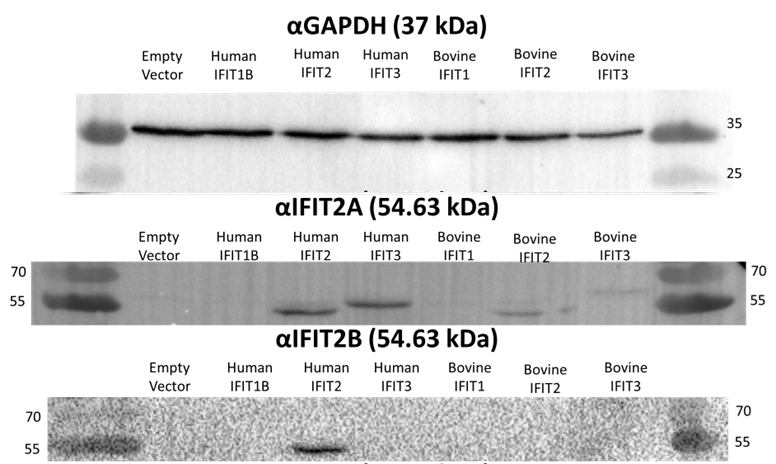
\includegraphics[width=1\linewidth]{10. Chapter 5//Figs//04. IFIT2AB Discussion/07. antibodies ifit2.png}
    \caption[ifit2 antibodies figure]{ifit2 antibodies figure}
    \label{fig:ifit2 antibodies figure}
\end{figure}

%Summary
We were thinking that the differential staining between IFIT2A and IFIT2B antibodies could be due epitope masking (due to e.g. RNA interaction; interaction with other IFITs; interaction with other cellular proteins; interaction with viral proteins) but although both of the antibodies seem to detect IFIT2 in western bots, they differ quite substantially in other aspects. One fails to capture induction caused by P transfection, while the other fails to capture kinetochore microtubule staining.
\subsection{Importance of RNA Binding} \label{subsec:Importance of RNA Binding}
\lipsum[1-3]